\documentclass[iop,twocolappendix]{emulateapj}
\usepackage{blindtext}
%\usepackage{float}
\usepackage{placeins}
\usepackage{graphicx}
\usepackage{amssymb, amsmath}
\usepackage{natbib}
\usepackage{amsmath}
\usepackage{bm}
\usepackage{color}
\usepackage[colorlinks,urlcolor=blue,citecolor=blue,linkcolor=blue]{hyperref}
%\usepackage{subfigure}
%\usepackage{caption}
%\usepackage{subcaption}
\interfootnotelinepenalty=10000
\usepackage[caption=false]{subfig}
\DeclareMathOperator{\sech}{sech}
\begin{document}
\title{The Mechanism of Electron Acceleration in trans-relativistic magnetic reconnection}

\author{David Ball,\altaffilmark{1,3} Lorenzo Sironi,\altaffilmark{2} and Feryal \"Ozel\altaffilmark{1}}

\altaffiltext{1}{Department of Astronomy and Steward Observatory, Univ. of Arizona, 933 N. Cherry Avenue, Tucson, AZ 85721, USA}

\altaffiltext{2}{Department of Astronomy, Columbia University, 550 West 120th Street, New York, NY 10027, USA}
\altaffiltext{3}{Email: davidrball@email.arizona.edu}

\begin{abstract}
We investigate electron acceleration mechanisms in a low-$\beta$ electron-proton plasma with moderate magnetization.  By varying the guide field and whether or not we trigger reconnection, we vary the number of x-points and plasmoids that form in a given simulation, which we show plays an important role in particle acceleration.  Specifically, we show that x-points, either in the primary current layer or in between merging plasmoids are a necessary first step to accelerate electrons out of the cold initial distribution to highly relativistic ($\gamma > 100$) energies.  Once an electron goes through this step, it can be further accelerated by different mechanisms that may be energetically dominant compared to the initial acceleration at an x-point, but the vast majority of the highly relativistic ($\gamma > 1000$) electrons across our set of simulations are first accelerated at an x-point.  As a result of this, the simulations with more x-points and plasmoids have harder electron spectra than the cases with fewer structures.


%Specifically, when no guide field is present, the secondary tearing mode is active and forms copious x-points and plasmoids.  X-points directly accelerate particles through a strong non-ideal field, while plasmoids merge and form current sheets in between them, which serve as sites of further acceleration. When less x-points and plasmoids form, either by suppressing the secondary tearing mode, o

%We further emphasize the effect of varying the number of x-points by comparing triggered and untriggered simulations. In an untriggered simulation there are more x-points and plasmoids than a triggered simulation with identical physical parameters.  Indeed, we find that the spectra from untriggered simulations are systematically harder than their triggered counterparts due to the increased number of x-points and plasmoid mergers.

\end{abstract}
\keywords{magnetic reconnection --- accretion, accretion disks ---galaxies: jets ---X-rays: binaries --- radiation mechanisms: nonthermal --- acceleration of particles} 
\maketitle

\section{introduction} \label{introduction}
Magnetic reconnection is thought to play an important role in accelerating electrons and powering high-energy emission in numerous astrophysical systems including blazar jets (citations), pulsar wind nebulae (citations), gamma ray bursts (citations), the Sun (citations), and accretion flows around black holes (citations).  Despite its ubiquity, the physics of particle acceleration through reconnection is not fully understood.  

Numerous studies have investigated electron acceleration mechanisms in both relativistic (\citealt{nalewajko2015}; \citealt{guo2015}; \citealt{werner2017}) and nonrelativistic reconnection (\citealt{dahlin2014}; \citealt{li_guo_2017}; \citealt{wangh2016}).  These studies generally take one of two approaches: some apply a guiding center formalism (e.g., \citealt{dahlin2014}) in which they can cleanly separate different acceleration mechanisms in the energy equation for a single particle and ultimately assess the various contributions solely by looking at cell averaged currents, velocities,  and fields. However, this formalism breaks down at x-points in anti-parallel reconnection, where the magnetic field vanishes.  Others look at individual particle trajectories to assess where and by what mechanisms particles are being accelerated.  However, these studies have so far sparsely sampled a collection of representative particles.  Furthermore, most of these studies employ either a pair-plasma or a significantly reduced mass ratio. 

These previous studies have highlighted a few distinct acceleration mechanisms.  One such mechanism is acceleration by the out-of-plane (i.e., in the direction of $\vec{\nabla} \times \vec{B}$) electric field at x-points (citations).  These x-points can occur not only in the in the initial current sheet via the primary or secondary tearing mode, but also in the current sheets generated between merging plasmoids, where reconnection also occurs.  Another prominent mechanism is Fermi reflection, enabled by the various macro-scale motions induced by reconnection.  Fermi reflection can occur between merging plasmoids (citations), within contracting plasmoids (citations), and also between outflows and plasmoids (citations).  \citet{nalewajko2015} also found that particles are accelerated in the trailing edges of plasmoids as they move.

In \citet{ball2018} we investigated particle acceleration in the trans-relativistic regime and found preliminary evidence for the role of x-points, plasmoids, and Fermi-type processes by examining the histories of a few representative high-energy particles.  We did not, however, examine a statistically meaningful sample of particles.  In that study, we observed that at low-$\beta$, electron acceleration is characterized by extremely short periods of intense acceleration by a non-ideal electric field at x-points in the initial sheet or between merging plasmoids.  In contrast, at high-$\beta$ when electrons start out relativistic, x-point acceleration is negligible, and Fermi reflection dominates.  The reason for this is twofold; first, the secondary tearing mode is suppressed at high-$\beta$; second, the energy gain via Fermi reflection off of features moving at the Alfv\'en speed dominates over the energy gain at x-points.

In this paper, we investigate the physical mechanisms of electron acceleration by comparing four simulations in which we vary the number of x-points and plasmoids by changing guide field strength and whether or not we trigger reconnection.  We address the issues of downsampling in time and particle number, as well as the reduced mass ratio by performing simulations with the realistic electron-proton mass ratio while including particle acceleration diagnostics that are calculated on-the-fly during the simulation for all of the particles.  We also employ robust methods of identifying x-points and track the role of the parallel and perpendicular electric field (relative to the local magnetic field) in order to investigate the detailed histories of the accelerated particles.  

We find that x-points and plasmoid mergers play critical roles in accelerating electrons in the trans-relativistic regime.  In particular, we find that when the secondary tearing mode is active, electron acceleration is significantly enhanced and occurs throughout the domain.  In these cases, x-points and plasmoid mergers are ubiquitous  and play comparable roles in accelerating electrons.  In contrast, when the secondary tearing mode is suppressed, high-energy acceleration is localized to the primary x-point(s) and the mergers of primary plasmoids, which are very few relative to the copious secondary x-points and plasmoids that occur when secondary tearing is active.


\section{methods} \label{methods}

\subsection{Simulation Setup} \label{sim_details}
We perform four fiducial simulations of magnetic reconnection using the publicly-available code TRISTAN-MP (\citealt{buneman93}; \citealt{spitkovsky05}).  We employ a two-dimensional (2D) simulation domain in the $xy$ plane, but we track all three components of velocity and electromagnetic field vectors.  We set up the system in Harris equilibrium, with a magnetic field profile $\bm{{B}} = -B_{0}\tanh{\left(2\pi y / \Delta\right)}\bm{\hat{x}}$, where $B_{0}$ is the strength of the reconnecting field in the ambient plasma and $\Delta$ is the thickness of the sheet.  $B_{0}$ is related to the magnetization parameter $\sigma$ via $\sigma=B_{0}^2 / 4\pi w_{0} $, where $w_{0}$ is the enthalpy density of the ambient plasma $w_0=(\rho_{e}+\rho_{i})c^{2}+ \hat{\gamma}_{e}u_{e}+ \hat{\gamma}_{i}u_{i}$, with $\rho_{i,e}$, $\hat{\gamma}_{i,e}$, and $u_{i,e}$ being the mass densities, adiabatic indices, and internal energy densities of ambient protons and electrons, respectively.  We include an out-of-plane magnetic field (referred to as a guide field) and specify its strength as a fraction of the reconnection component, $B_{g}/B_{0}$.  We specify the temperature through the proton $\beta$, defined as $\beta \equiv \beta_{i}=8 \pi n_{i} k T_{i}/B_{0}^{2}$, where $n_i=\rho_i/m_i$ is the proton number density, $T_i$ is the proton temperature, and $m_i$ is the proton mass. Ambient electrons and protons start with the same temperature, so $\beta_e=\beta_i=\beta$ (the total plasma beta, including both species, is $2\,\beta$). In our low-$\beta$ case of $\beta_{i}=0.003$, the ambient protons are non-relativistic, so the magnetization parameter as defined with the proton rest mass $\sigma_i=B_0^2/4\pi \rho_i c^2$ is nearly identical to the enthalpy-weighted magnetization $\sigma$ defined above. Each computational cell in the ambient plasma is initialized with four particles per cell ($N_{ppc}=4$). 

\subsection{Parameter Scans}

\begin{figure*}[!h]
	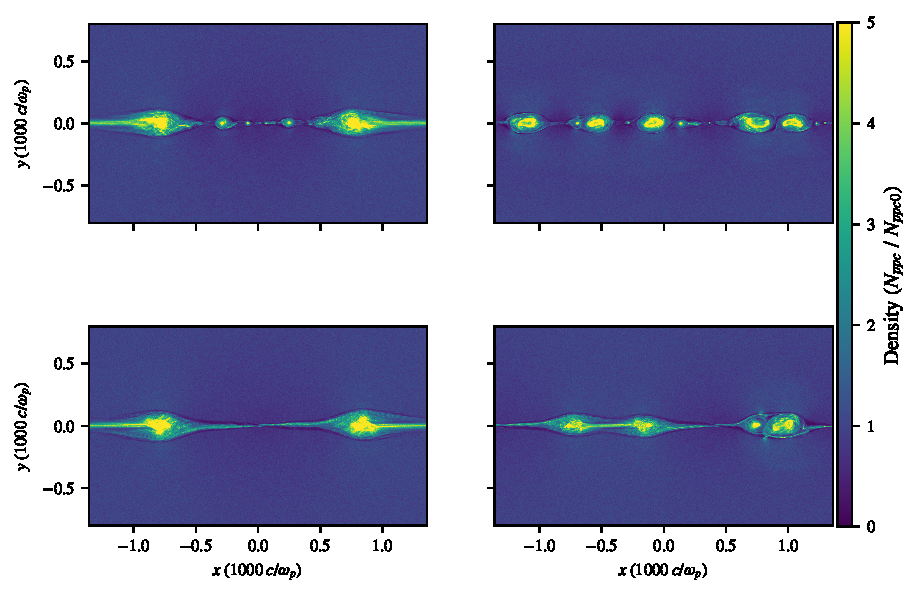
\includegraphics[width=\linewidth]{2x2_flds.pdf}
	\caption{Snapshots of density from our four fiducial simulations.  The left column shows the simulations with zero guide field and the right column shows the simulations with a guide field.  The first row shows simulations where reconnection is triggered by hand, and the second row shows simulations where reconnection develops spontaneously, resulting in more plasmoids than their triggered counterparts.
	}
	\label{lowbeta_fourdens}
\end{figure*}


Our goal in investigating the acceleration mechanism is to create density and field structures that are drastically varied and examine how this affects particle acceleration.  We find that one numerical and one physical parameter can control the structure of the current sheet and give us a great diversity of current layers just by changing the simulation setup and guide field strength.  Specifically, for our particular values of $\sigma$ and $\beta$, when we include a guide field of strength $B_{g}/B_{0}=0.3$, it effectively suppresses the formation of x-points and plasmoids.  Additionally, by triggering reconnection or allowing it to evolve spontaneously, we can alter the number of x-points and plasmoid mergers.

We show snapshots from our four simulations in Figure \ref{lowbeta_fourdens}.  Here, the top row shows snapshots of density from the simulations of purely anti-parallel reconnection while the bottom row shows snapshots from simulations with $B_{g}/B_{0}=0.3$.  The left column shows the triggered simulations while the right column shows the untriggered simulations.  We see that, for the particular $\sigma$ and $\beta$ we use here, a guide field with strength $B_{g}/B_{0}=0.3$ increases the width of the current layer and results in thicker, more stable current sheets that do not fracture via the secondary tearing mode.  This is in stark contrast with anti-parallel simulations at the same $\sigma$ and $\beta$ (top row), where the current sheet fractures copiously into x-points and plasmoids.
 
All PIC studies of reconnection have to make the choice of whether to trigger reconnection at specific point in the current sheet or to let it evolve spontaneously, but the implications of this choice are not fully understood.  In a triggered setup there is one primary x-point and the Alfv\'en crossing time is greater than the primary tearing timescale.  Because of this, a single large magnetic island forms at the boundary when the reconnection fronts collide, and no other primary plasmoids form.  Instead, in the region vacated by the reconnection fronts, the secondary tearing mode (when active) forms x-points and plasmoids in the center of the domain which are pulled to the edges of the box and ultimately merge with the large boundary island.  In contrast, in an untriggered setup, numerous primary x-points and plasmoids form via the primary tearing mode.  These primary plasmoids then hierarchically merge until there is one large magnetic island.  In this way, the untriggered setup invariably has more primary x-points as well as more large plasmoid mergers than a triggered setup with the same physical parameters.  One can make arguments for the applicability of either choice to realistic situations.  However, here we utilize both as a numerical tool to achieve a diversity of density and electromagnetic field structures to enable us to track electron acceleration under these varied conditions.


\section{Diagnostics of Acceleration}
In this section, we describe how we explore the acceleration mechanisms through a combination of tracking particle acceleration histories as well as identifying x-points from the structure of the electromagnetic fields.  In subsection \ref{diagnostics}, we describe the properties of particles that we track that inform our understanding of their acceleration history.  In \ref{xpoint_id}, we describe our method for identifying x-points from the structure of the magnetic field.  Finally, in \ref{acc_mec_def}, we define the criterion we employ to associate acceleration episodes with either x-points or mergers.
\subsection{Tracking Particle Properties} \label{diagnostics}
In \citet{ball2018}, we found that electrons generally experience extremely short episodes of acceleration, characterized by sudden jumps in their energy, rather than a steady and continuous energy gain.  This presents a problem in accurately identifying the time and location of particle acceleration episodes because the output cadence is often drastically down-sampled in time from the actual simulation timesteps.  In other words, by the time the simulation produces an output file, the particle may have moved significantly from where it was accelerated, and we lose the ability to accurately identify where and when the particle was accelerated.  In addition, particle outputs are also typically down-sampled in number due to the large number of particles necessary for PIC simulations.  Typically only a small fraction of particles are saved in the output files for analyzing. 

In order to get around these problems, we track three additional properties of the particles.  These properties are the time and location of the particle when its Lorentz factor $\gamma$ first exceeds $\sigma_{e}/2$.  We call this time and location $t_{cs}$ and $x_{cs}$, respectively.  We also keep track of the maximum value of $E_{z}/B_{xy}$ that the particle experiences up to the point where it exceeds the above criterion.  Here, $E_{z}$ is the out-of-plane electric field and $B_{xy}=(B_{x}^{2}+B_{y}^{2})^{1/2}$ is the in-plane magnetic field.  This quantity is a useful diagnostic of particle acceleration: regions with high magnetic dissipation where non-ideal fields are present will have have $E_{z}/v_{A}B_{xy}>1$, where $v_{A}$ is the Alfv\'en speed.  By checking for the $\gamma > \sigma_{e}$ condition at every simulation timestep and recording the time and position when this criterion is satisfied, we overcome the time-downsampling problem mentioned previously.  Additionally, we track and analyze these properties for all of our particles, not just a downsampled selection.  We note, however, that this method will only capture the first acceleration episode that a particle experiences.  This first episode, however, is critical to promoting the electron to relativistic energies, where it can then sample large-scale velocity differences and become further energized through Fermi-type processes.  In order to explore acceleration after the particle's promotion out of the cold $\gamma\approx1$ population to highly relativistic velocities, we also follow a sample of particle trajectories and explore the relative contributions of $E_{||}$ and $E_{\bot}$ (the parallel and perpendicular components of the electric field to the magnetic field) to the energization of a particle.  In general, we find that particles are almost always first accelerated by $E_{||}$ at an x-point, and then are further accelerated by a combination of $E_{||}$ in current sheets during plasmoid mergers and $E_{\bot}$ in the interaction of outflows with plasmoids and the dissipation of turbulent motions within plasmoids.


\subsection{X-point Identification} \label{xpoint_id}
%In order to associate electron energization episodes with x-points, we first identify x-points from the cell averaged fields.  X-points correspond to local minima in the z-component of the magnetic vector potential, $A_{z}$, while plasmoids correspond to local maxima.  As such, in order to identify x-points in the current sheet, we calculate the z-component of the magnetic vector potential in a slice along the midplane where the current sheet resides.  We then identify local minima with a simple algorithm: we iterate through every point along the slice, if the value of $A_{z}$ is smaller at this point than it is at any points within $\pm S$ cells, then we consider this an x-point.  We have experimented with the optimal value for $S$, this distance to either side of a point we search for minima, and found that a value of $\sim 20\; c/\omega_{p}$ is sufficient for the typical distance between x-points we see in our simulations.  We note that this algorithm will systematically miss x-points if their separation $< S$.  
In order to test the association of electron energization episodes with x-points, we first identify x-points from the cell averaged fields.  \citet{haggerty2017} recently studied the statistics of x-points in turbulence via PIC simulations and explored methods to robustly identify x-points.  In a 2.5D setup such as ours, x-points correspond to saddle points in the z-component of the magnetic vector potential, $A_{z}$.  Following \citet{haggerty2017}, we first apply a Gaussian filter with a width of $\sim 4 \; c/\omega_{p}$ to the z-component of the magnetic vector potential, $A_{z}$.  We then identify critical points where $\partial A_{z}/\partial x=\partial A_{z}/\partial y=0$.  In order to distinguish between local minima, maxima, and saddle points, we calculate the matrix of second derivatives (or, Hessian matrix), 
$$H_{ij}=\frac{\partial^{2} A_{z}}{\partial x_{i} \partial x_{j}}.$$  If the eigenvalues of this matrix are negative, this corresponds to a maximum in $A_{z}$, if both are positive, it corresponds to a minimum.  If, however, the eigenvalues are of opposite sign, then this is a saddle point and we identify it as an x-point.  We show in Figure \ref{xpoint_finding} a snapshot from our untriggered simulation with a guide field, where a large plasmoid merger occurs at the end of the simulation.  We plot the locations of x-points identified with the method described above with red x's.  We see that we are able to identify x-points not only the initial horizontal current sheet, but also x-points generated in the current sheets at the interface of merging plasmoids.


 \begin{figure}[htp]
 	
 	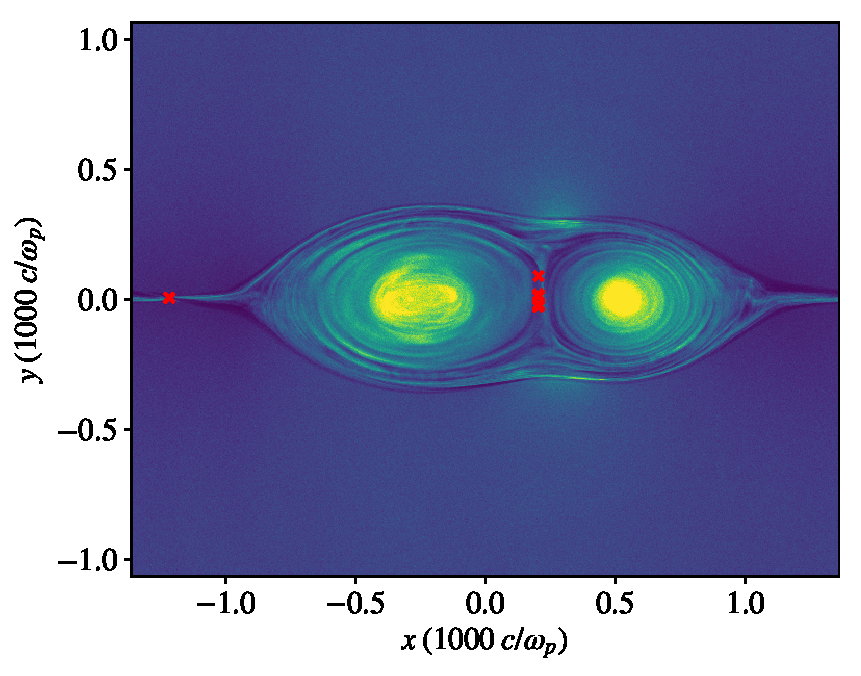
\includegraphics[width=\linewidth]{xpoint_finding.pdf}
 	\caption{Snapshot of density from an untriggered simulation showing a large plasmoid merger as well as an x-point in the horizontal current sheet.  We show with red X's where the x-point identification algorithm picks out x-points at this snapshot.  We see we are able to successfully identify x-points in both the horizontal and vertical current sheets.}
 	\label{xpoint_finding}
 \end{figure}


\subsection{Distinguishing Criteria for Acceleration Mechanisms} \label{acc_mec_def}
We use a few simple criteria to distinguish between particles that are accelerated near an x-point in the initial horizontal current layer from those at the interface of two merging plasmoids.
If a particle is accelerated at an x-point in the initial horizontal current layer, then we expect the particle to be suddenly accelerated by a non-ideal out-of-plane electric field in the direction of $\vec{\nabla} \times \vec{B_{0}}$ when it enters the current layer at an x-point.  Reconnection also occurs in vertical current sheets formed between merging plasmoids where particles may also be accelerated.  A particle that is accelerated in a merging event will likely first interact with the current sheet by entering a plasmoid.  During this process, the particle will be heated due to the compression while the plasmoid forms.  The plasmoid will then merge with another plasmoid in the current layer, developing a vertical current sheet between them.  The sign of the electric field in these vertical current layers associated with mergers, however, is in the opposite direction from x-points in the initial layer (i.e., in the direction of $-\vec{\nabla} \times \vec{B_{0}}$).  

We illustrate this in Figure \ref{blines}, where we show in-plane magnetic field lines superimposed on a snapshot of density from the triggered simulation with a guide field.  We see a typical x-point in the horizontal current layer, highlighted by a cyan box.  Note that $\vec{\nabla} \times \vec{B}$ in this region is in the $+\hat{z}$ direction.  At $x\approx0.6$ we see a secondary plasmoid merging into the large boundary island.  A vertical current sheet forms and reconnection proceeds, with $\vec{\nabla} \times \vec{B}$  in the $-\hat{z}$ direction.

\begin{figure*}[!h]
	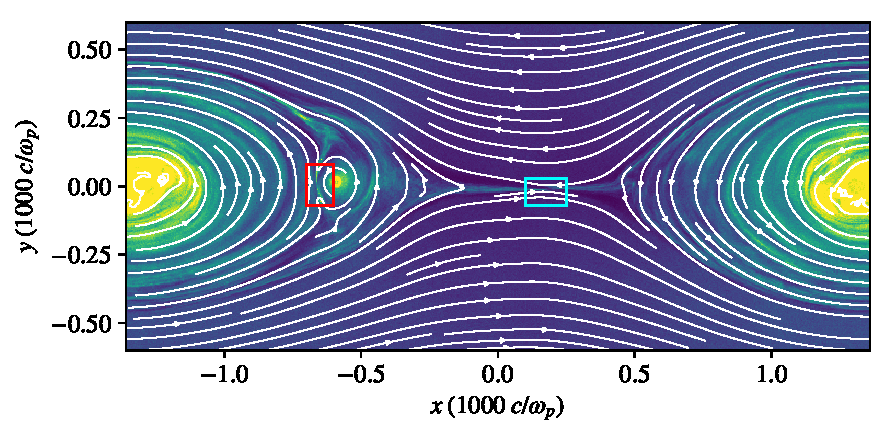
\includegraphics[width=\linewidth]{testing_blines.pdf}
	\caption{Snapshot of density from a triggered simulation with a guide field.  We superimpose streamlines of the in-plane magnetic field and emphasize two regions: the cyan box where reconnection is taking place in the initial horizontal current layer, and the red box, where reconnection is occurring between two merging plasmoids.  Note that the sign of $\vec{\nabla}\times \vec{B}$, and hence the sign of the electric field is positive in the horizontal layer (cyan box), and negative in the vertical current layer between plasmoids (red box).
	}
	\label{blines}
\end{figure*}



To find all the particles at a given time that are accelerated by x-points, we first identify x-points from the fields as described above in \ref{xpoint_id}.  Generally, after a particle is accelerated at an x-point, it either enters a plasmoid or an outflow and moves away from the x-point.  The outflow moves at $\sim v_{A}$, while plasmoids generally move slower than this; the maximum speed that particles move away from x-points is $\sim v_{A}$.  Because of that, we look for all particles that have acceleration episodes that are Alfv\'enically connected to an x-point, i.e., we require that 

\begin{equation}
\lvert\frac{x_{cs} - x_{xpoint}}{t_{cs}-t_{xpoint}}\rvert \le v_{A}.
\end{equation}

In order to identify particles that are associated with mergers, we exploit the geometry of reconnection at the interface of merging plasmoids.  As mentioned above, in a plasmoid merger, the sign of the electric field will be opposite that in the horizontal current layer's x-points. As such, if the $E_{z}$ field is negative at the time of a particle's acceleration, we identify the acceleration episode as being due to a merger.

If neither of the above criteria are met, we classify the episode as ``other''.  We find that these uncategorized episodes generally produce much lower-energy particles than x-points or mergers, and they are often associated with plasmoid motion, contraction, or the interaction of an outflow with a plasmoid.  

%\begin{figure}[b]
%	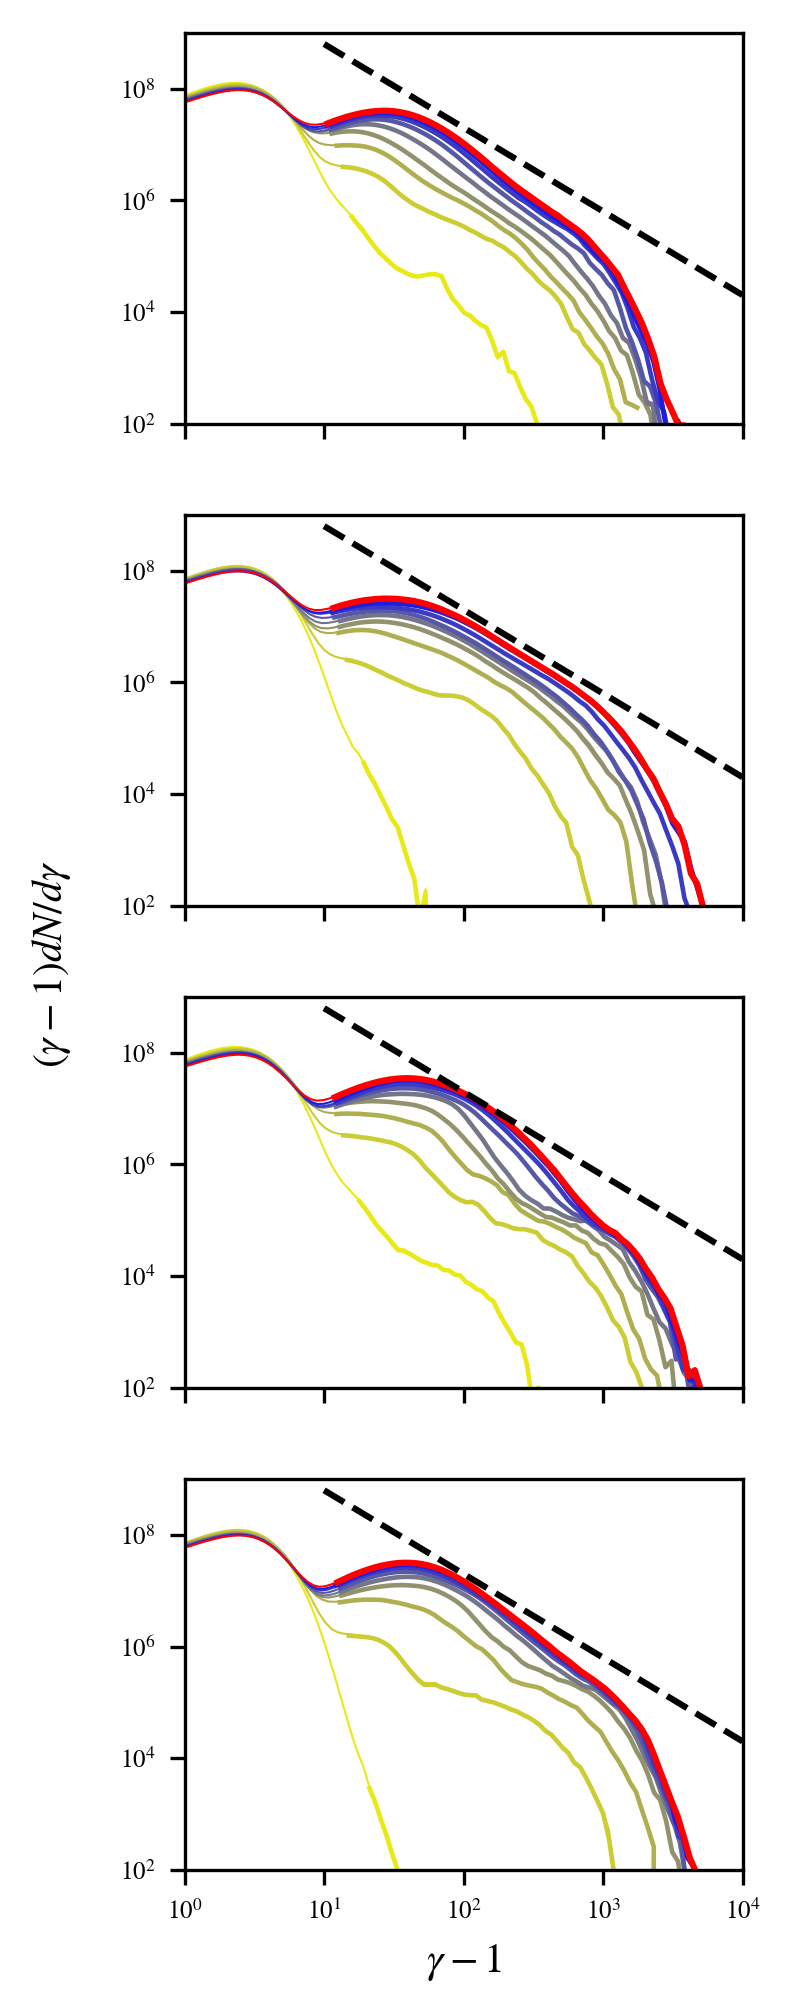
\includegraphics[width=.95\linewidth]{4x1_timespec.png}
%	\caption{Time evolution of the electron energy spectra from our four fiducial simulations, shown in the same order as in Figure \ref{lowbeta_fourdens}.  Time increases from yellow to blue, and the red line depicts the spectra from the final timestep.  We see that the untriggered zero guide field case has the hardest spectra, consistent with the fact that this simulation has the most x-points and plasmoid mergers.
%	}
%	\label{4x1_timespec}
%\end{figure}

%While investigating how the presence of a guide field affects the structure of the reconnection layer in the trans-relativistic regime (a forthcoming study), we found that guide fields suppress secondary plasmoid formation at low-$\beta$.  In short, the guide field decreases the compressibility of the upstream plasma, resulting in a less dense and thicker current sheet.  The tearing mode depends sensitively on the thickness of the sheet, with thicker sheets being more stable, so the presence of even a modest guide field in this regime stabilizes the current sheet against the tearing instability.  We will defer a more detailed analysis of this to a forthcoming study.  

%We are interested in examining the role of x-points as sites of particle acceleration.  Because of this, it is prudent to have a method of controlling the number of x-points in a simulation, and the guide field allows us to do just that.  Another way we can vary the number of x-points in a given simulation is to trigger reconnection at a specified location in the initial current sheet by removing the thermal support by hand, causing a local collapse of the layer, rather than letting the tearing mode develop spontaneously by particle noise.

%We show a snapshot of density from our four simulations with $\sigma=0.3$ and $\beta=0.003$ in Figure \ref{lowbeta_fourdens}.  The top two panels show our simulations with zero guide field, while the bottom two panels depict the simulations with our guide field of strength $B_{g}/B_{0}=0.3$.  The first and third panels correspond to triggered simulations, while the second and fourth panels are untriggered.  We see that in the case of purely anti-parallel reconnection (top two panels) that numerous secondary x-points and plasmoids form: the current sheet is fractured by the secondary tearing mode into a plethora of secondary structures.  Additionally, we see that the untriggered simulations (second and fourth panels) have more x-points and larger plasmoids than their triggered counterparts.  


%In order to investigate the roles of x-points and plasmoid mergers as sites of particle acceleration we run four fiducial simulations with the additional particle acceleration diagnostics mentioned in the previous section.  These four simulations all have $\sigma = 0.3$ and $\beta=0.003$.  In two of the simulations, we trigger reconnection with a perturbation at the center of the box, whereas in the other two we allow the primary tearing mode to spontaneously occur, resulting in more x-points.  We include a guide field with a strength of $B_{g}/B_{0}=0.3$ in one triggered simulation and one untriggered simulation.  The remaining triggered and untriggered simulations are purely anti-parallel reconnection (no guide field).  We show the spectra from these simulations below in Figure \ref{4x1_timespec}.


\section{Acceleration Results}
In order to assess the relative importance of x-points and plasmoid mergers to the overall electron energy spectra, we iterate through time over all of our simulations and examine the cumulative spectra from the different acceleration mechanisms.  That is, at each output timestep, we identify the location of x-points as described in Section \ref{xpoint_id}.  We then associate all the particles with an acceleration mechanism as described in Section \ref{acc_mec_def}.  We then construct time-integrated energy spectra from these different components and assess their relative importance.  %n the following subsections, we show three representative snapshots for each of our four simulations, visually depicting how our algorithm is classifying different mechanisms, and finally we show time-integrated spectra for each component of acceleration. 

\begin{figure}[htp]
	{
		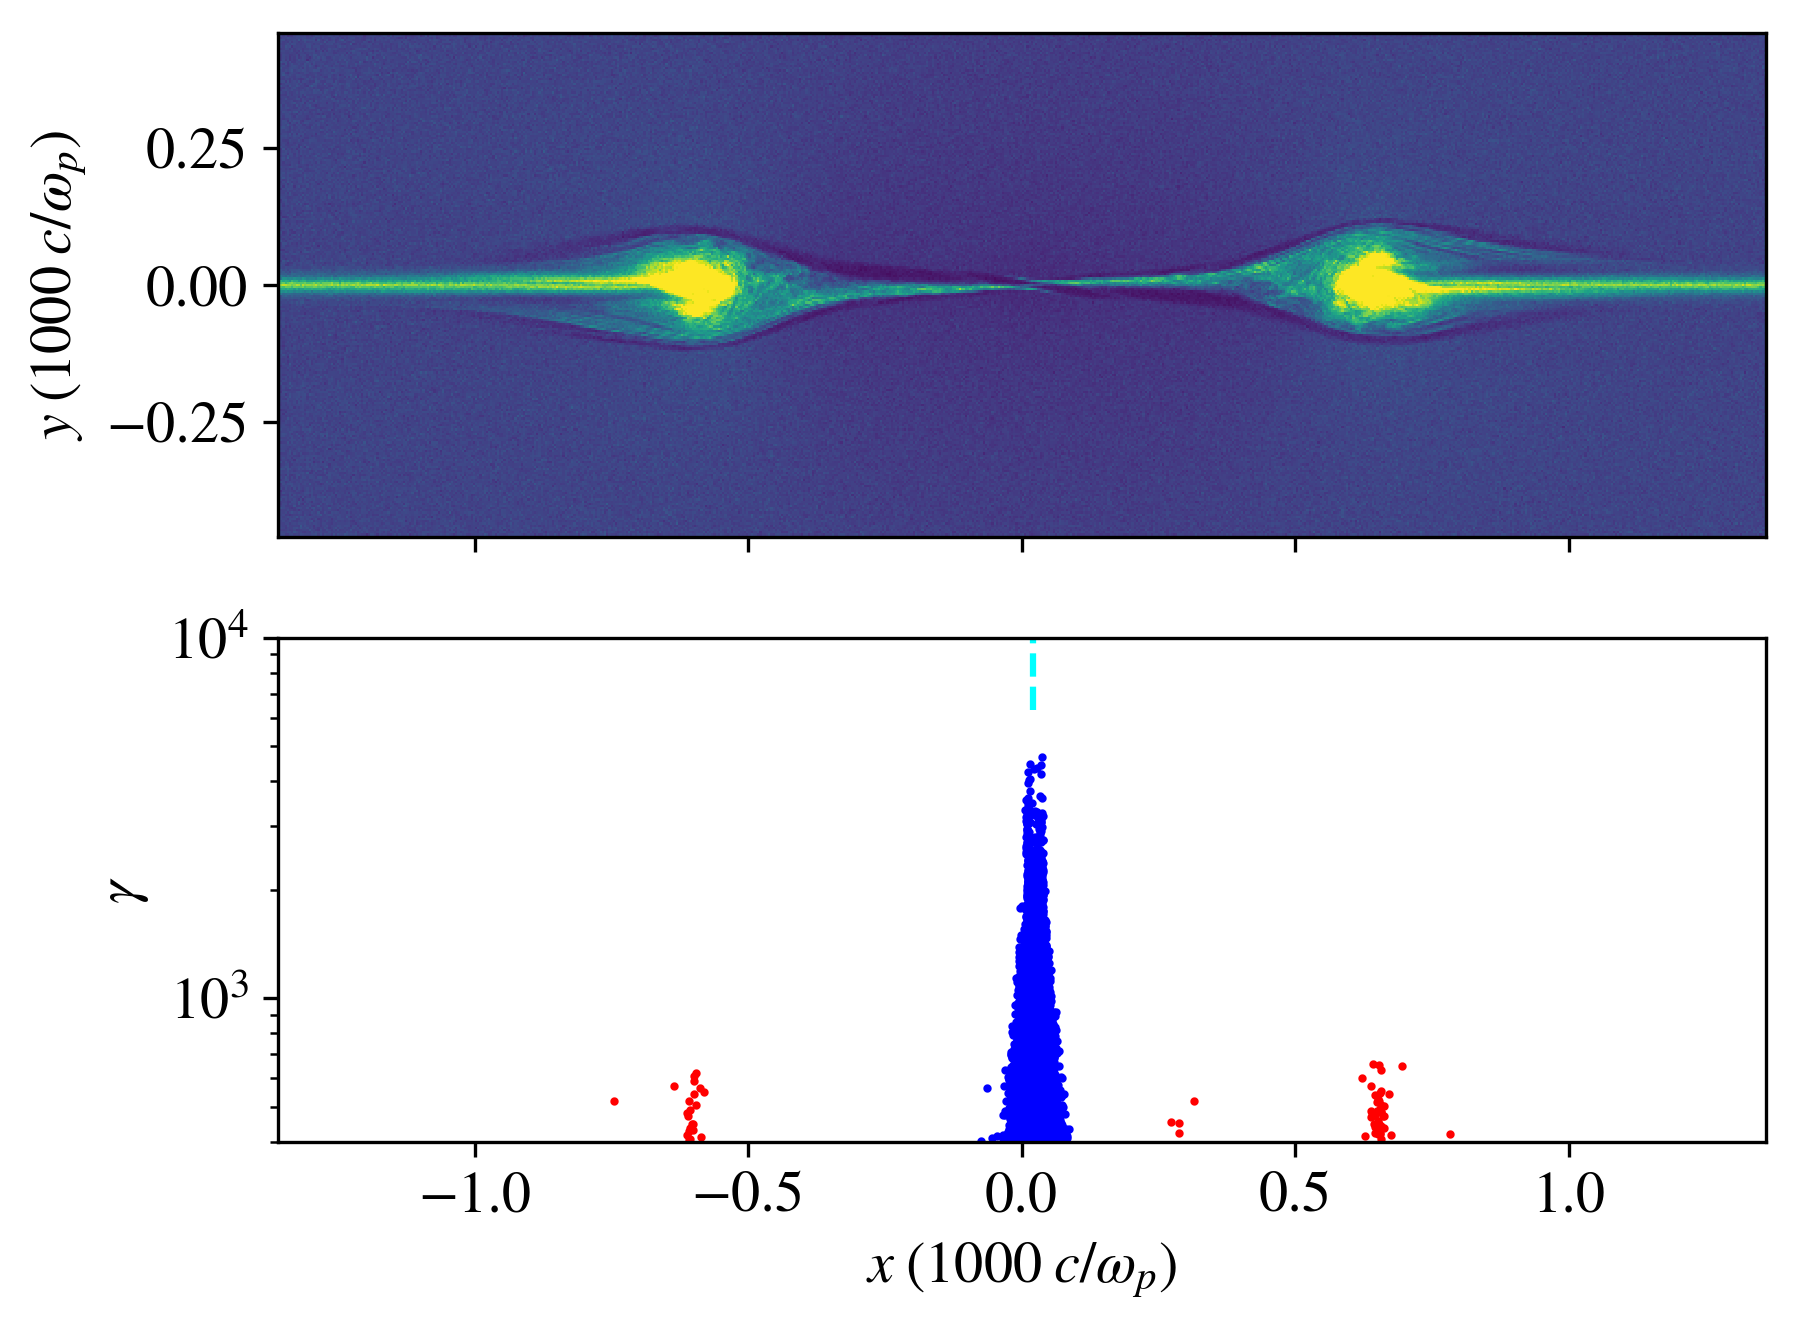
\includegraphics[width=\linewidth]{triggered_bguide_snapshot10.png}
	}
	\newline
	{
		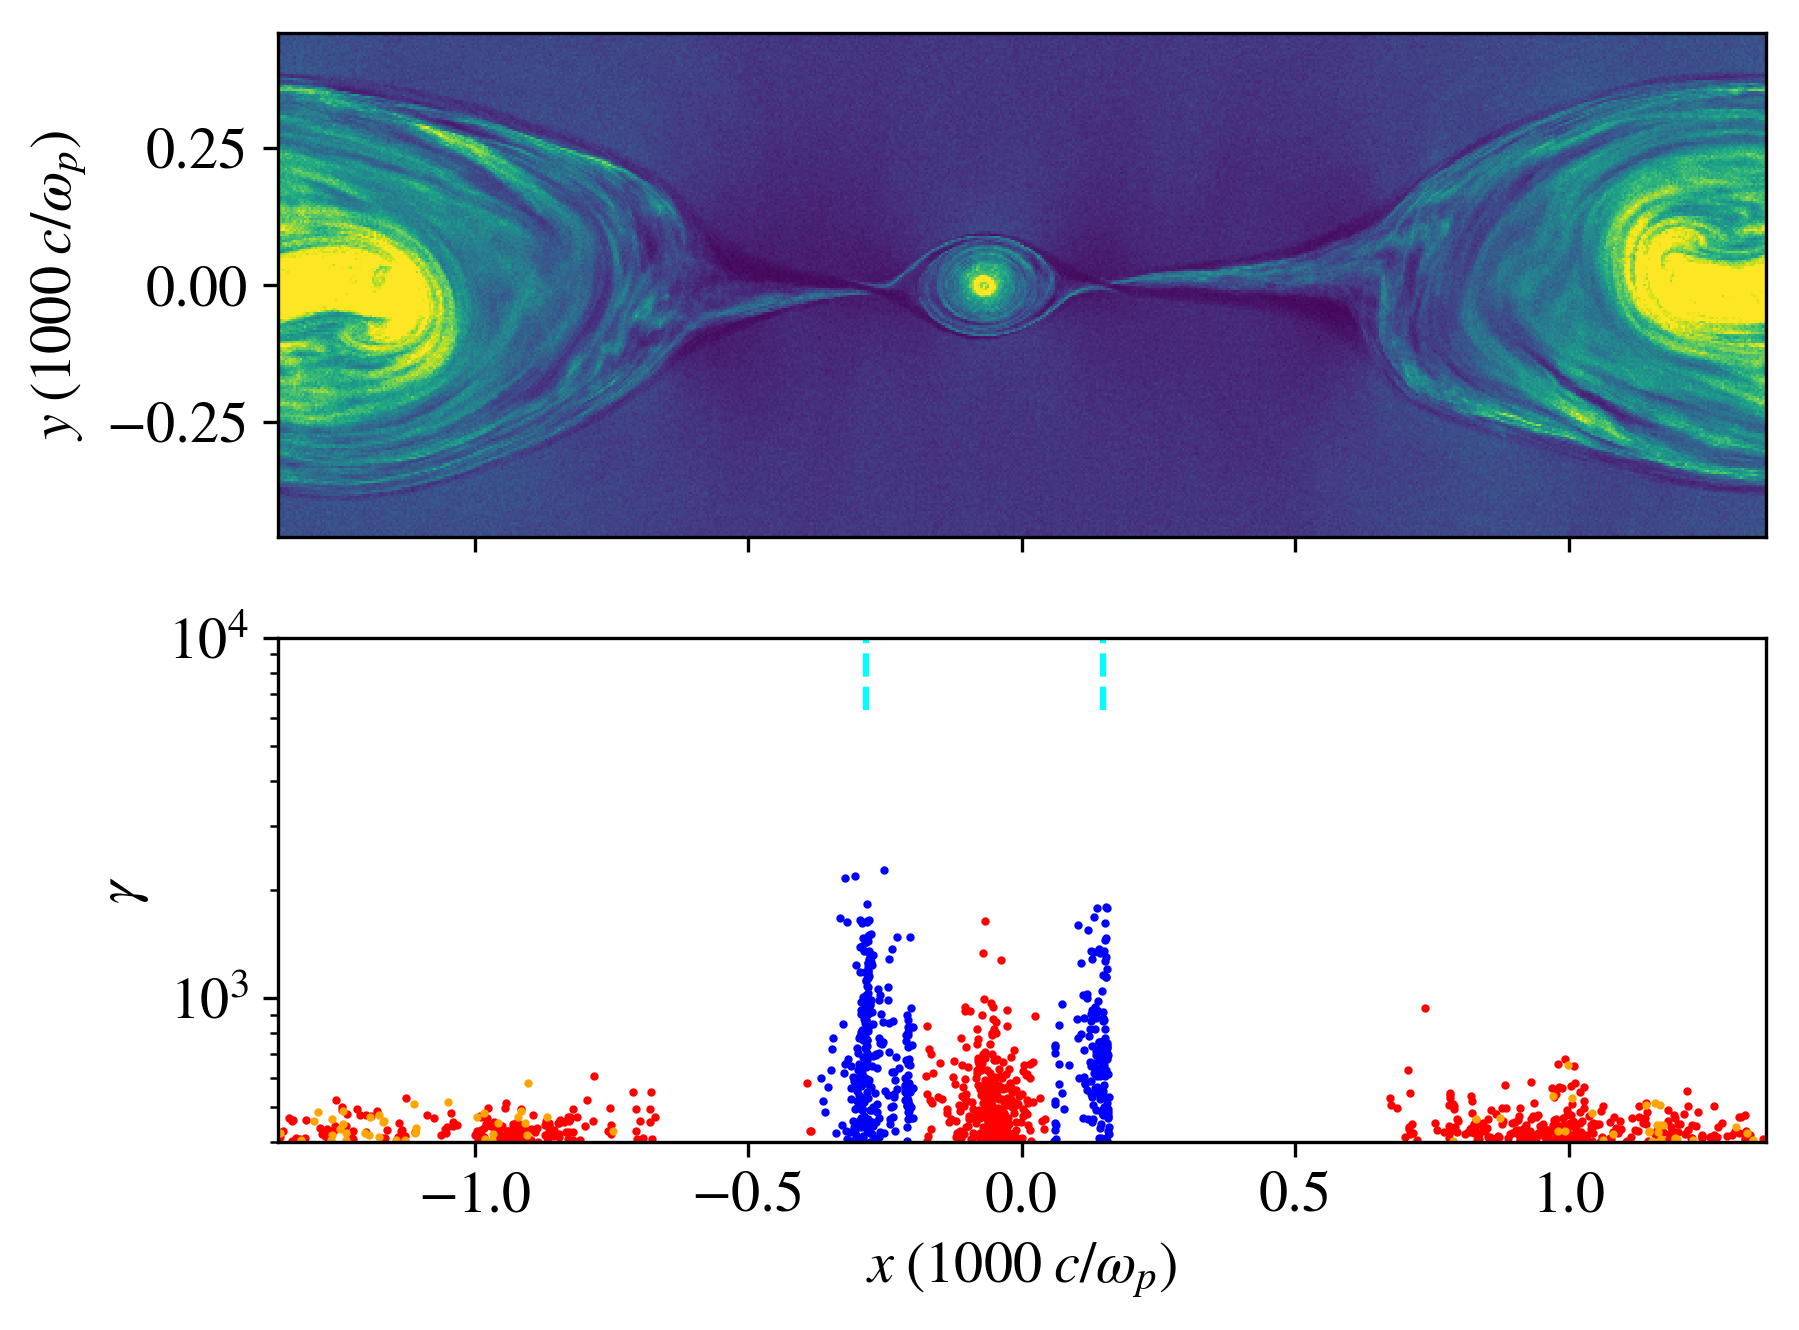
\includegraphics[width=\linewidth]{triggered_bguide_snapshot35.png}
	}
	\newline
	{
		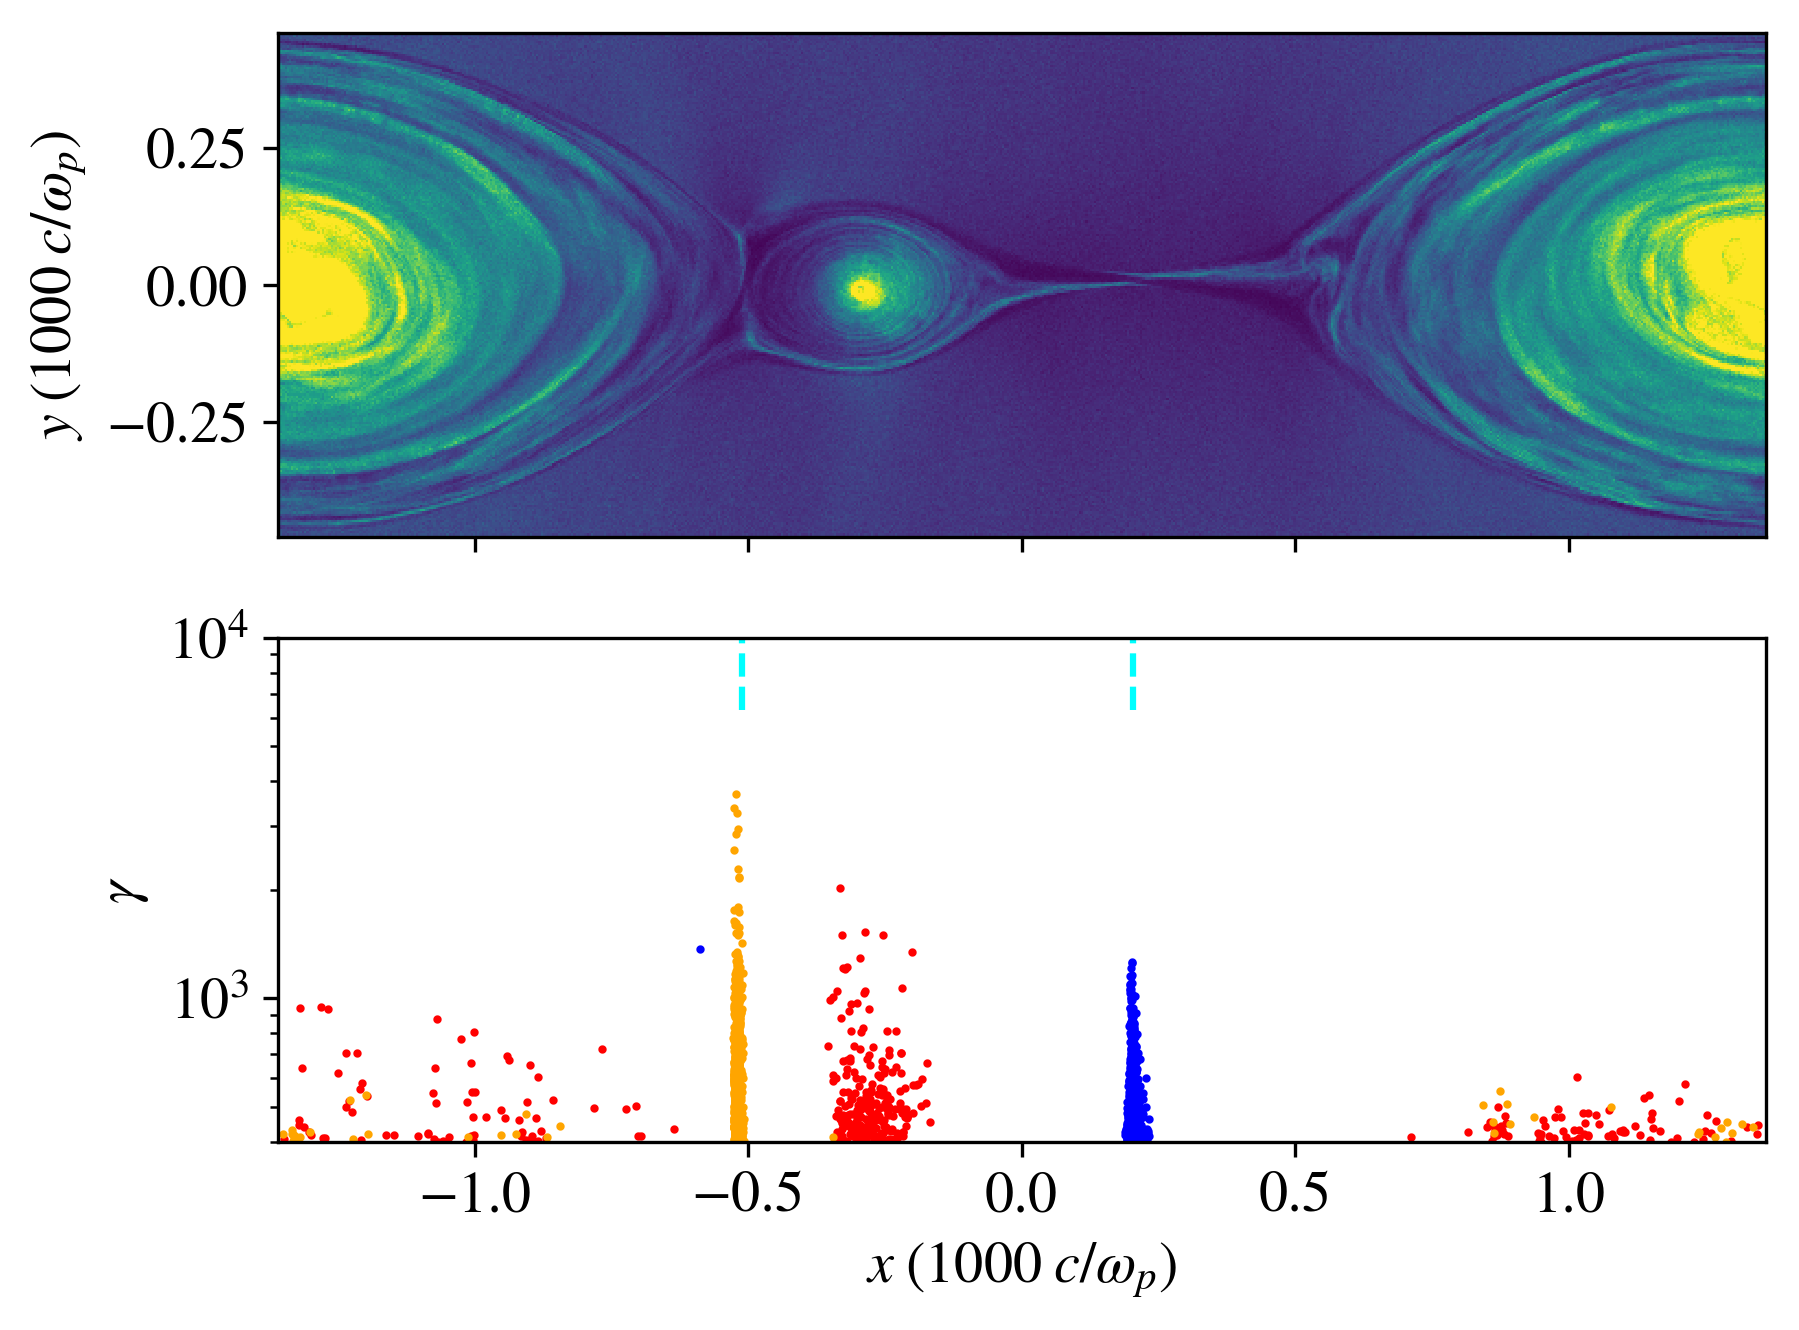
\includegraphics[width=\linewidth]{triggered_bguide_snapshot45.png}
	}
	
	\caption{Snapshots at three different times from the triggered simulation with a guide field strength of $B_{g}=0.3B_{0}$.  X-points are the dominant sites of electron acceleration and there are very few of them throughout the simulation.  One secondary plasmoid forms (middle panel), and eventually merges into the boundary island (bottom panel), which also accelerates some particles.
	}
	\label{triggered_bguide_snapshots}
\end{figure}


\begin{figure}[htp]
	
	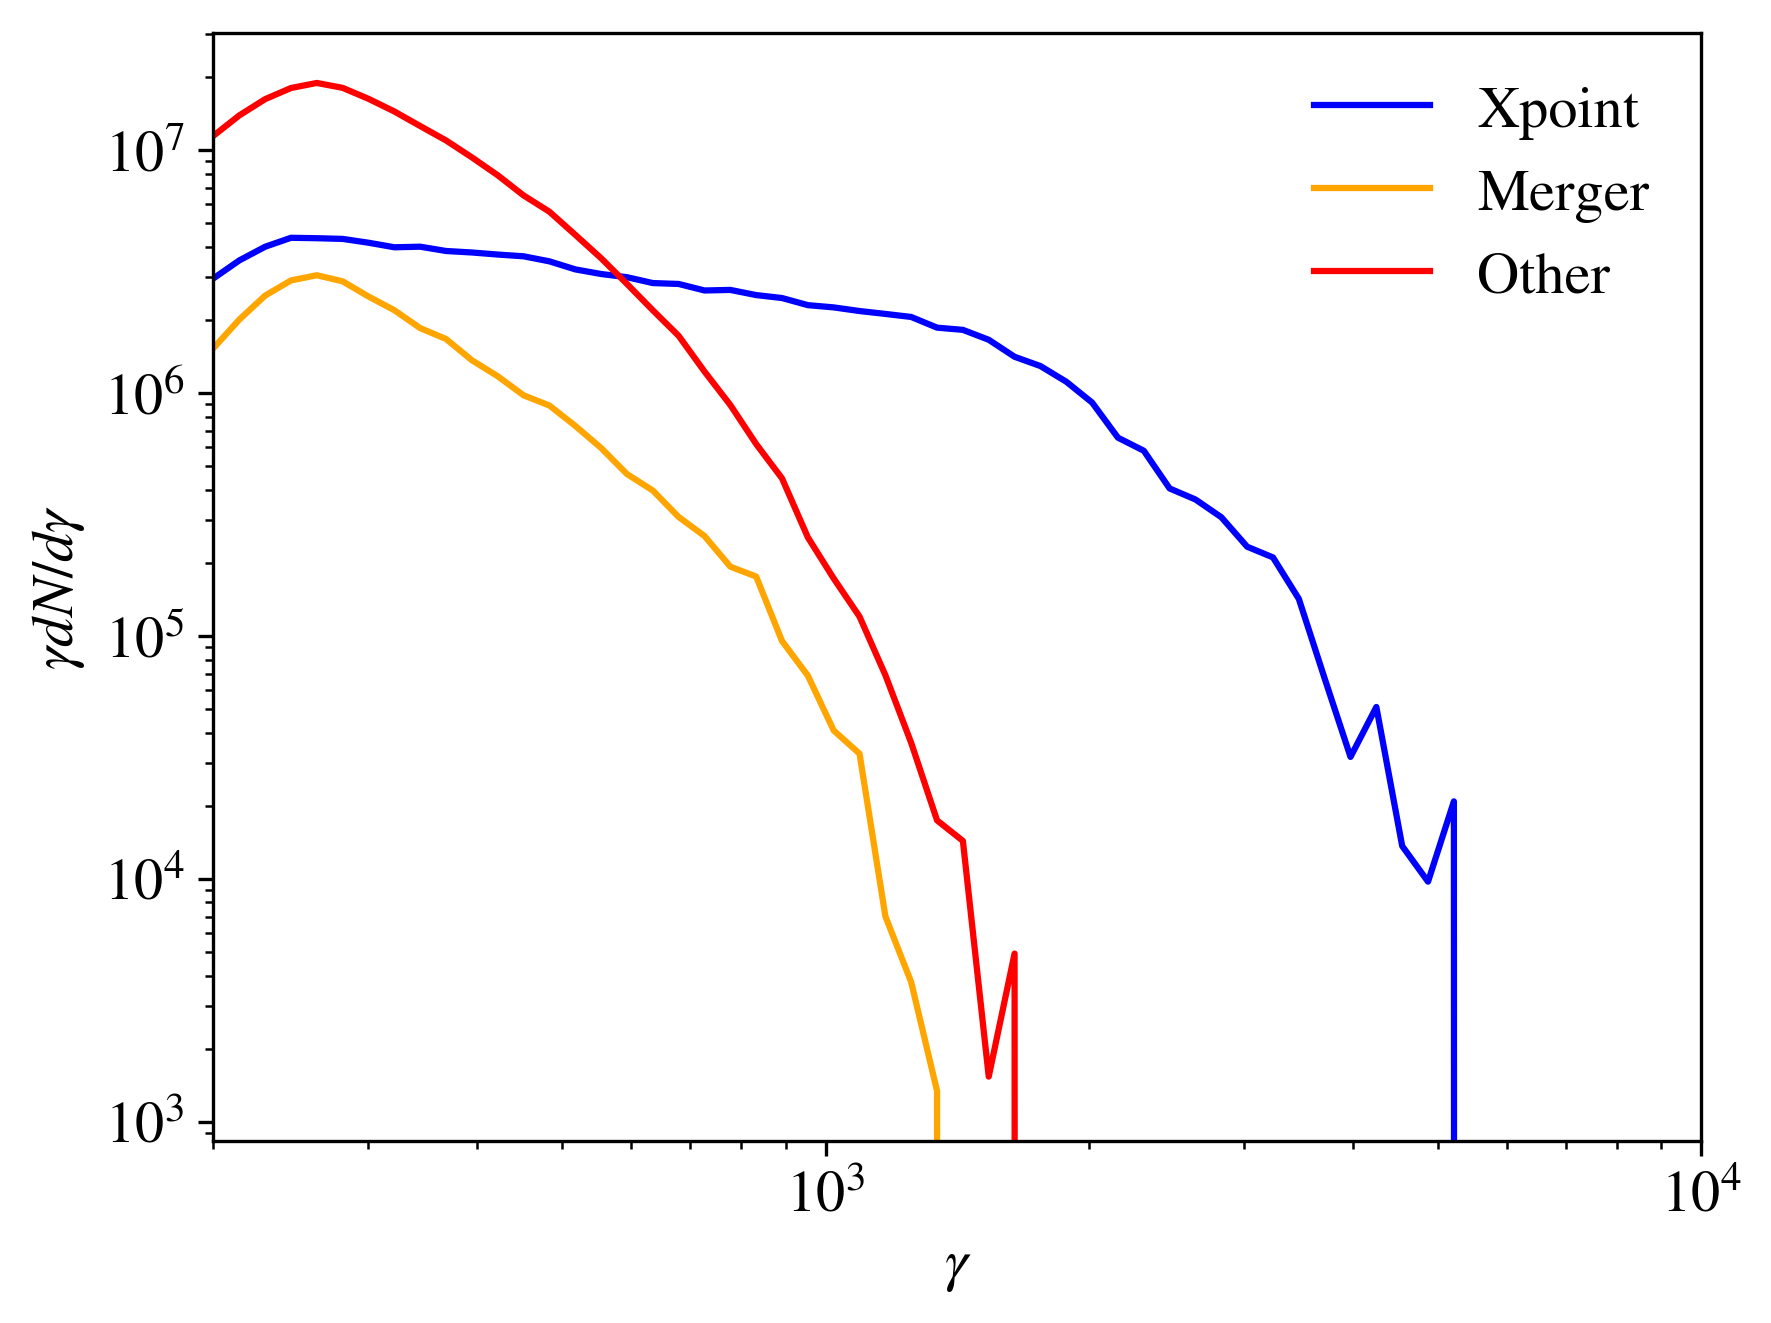
\includegraphics[width=\linewidth]{8k_bguide_triggered_stride1_2thresh_accmec_spect.png}
	\caption{Time-integrated electron spectra from the triggered simulation with guide field decomposed by acceleration mechanism.  X-points dominate all of the highest-energy electron acceleration.}
	\label{triggered_bguide_spec}
\end{figure}


We show in Figure \ref{triggered_bguide_snapshots} three snapshots in time from the triggered simulation with a guide field strength of $B_{g}=0.3B_{0}$, where the secondary tearing mode is suppressed.  Each timestep is depicted with two panels: the top panel shows the density profile, and the bottom panel depicts the location where the particle first exceeds $\sigma_{e}/2$ versus the particle's final energy. 

We see that at an early time (top two panels), there is a single primary x-point accelerating particles to high energies.  As reconnection proceeds, a single secondary plasmoid begins to develop in the middle of the domain (middle two panels), and there are two corresponding secondary x-points on either side.  These secondary x-points accelerate particles, but not as prolifically as the initial primary x-point.  Eventually, the plasmoid is pulled towards the left edge of the domain (bottom two panels) and merges with the large boundary island.  A current sheet forms between the two plasmoids and their magnetic fields reconnect, serving as another site of acceleration, with the expected flip in $E_{z}$ polarity from the x-points in the initial current sheet.  

We show the time-integrated spectra from the different mechanisms in Figure \ref{triggered_bguide_spec}.  In this case, almost all the highest energy particles ($\gamma > 1000$) come from x-points, and in particular, the primary x-point.  This is because the guide field suppresses secondary plasmoid formation, resulting in only one merging event over the course of the simulation.  We note that because acceleration is so localized in this case, in the limit of very large domains, the acceleration region will comprise a vanishing fraction of the total domain and we expect acceleration to be negligible.  

\begin{figure}[!h]
	{
		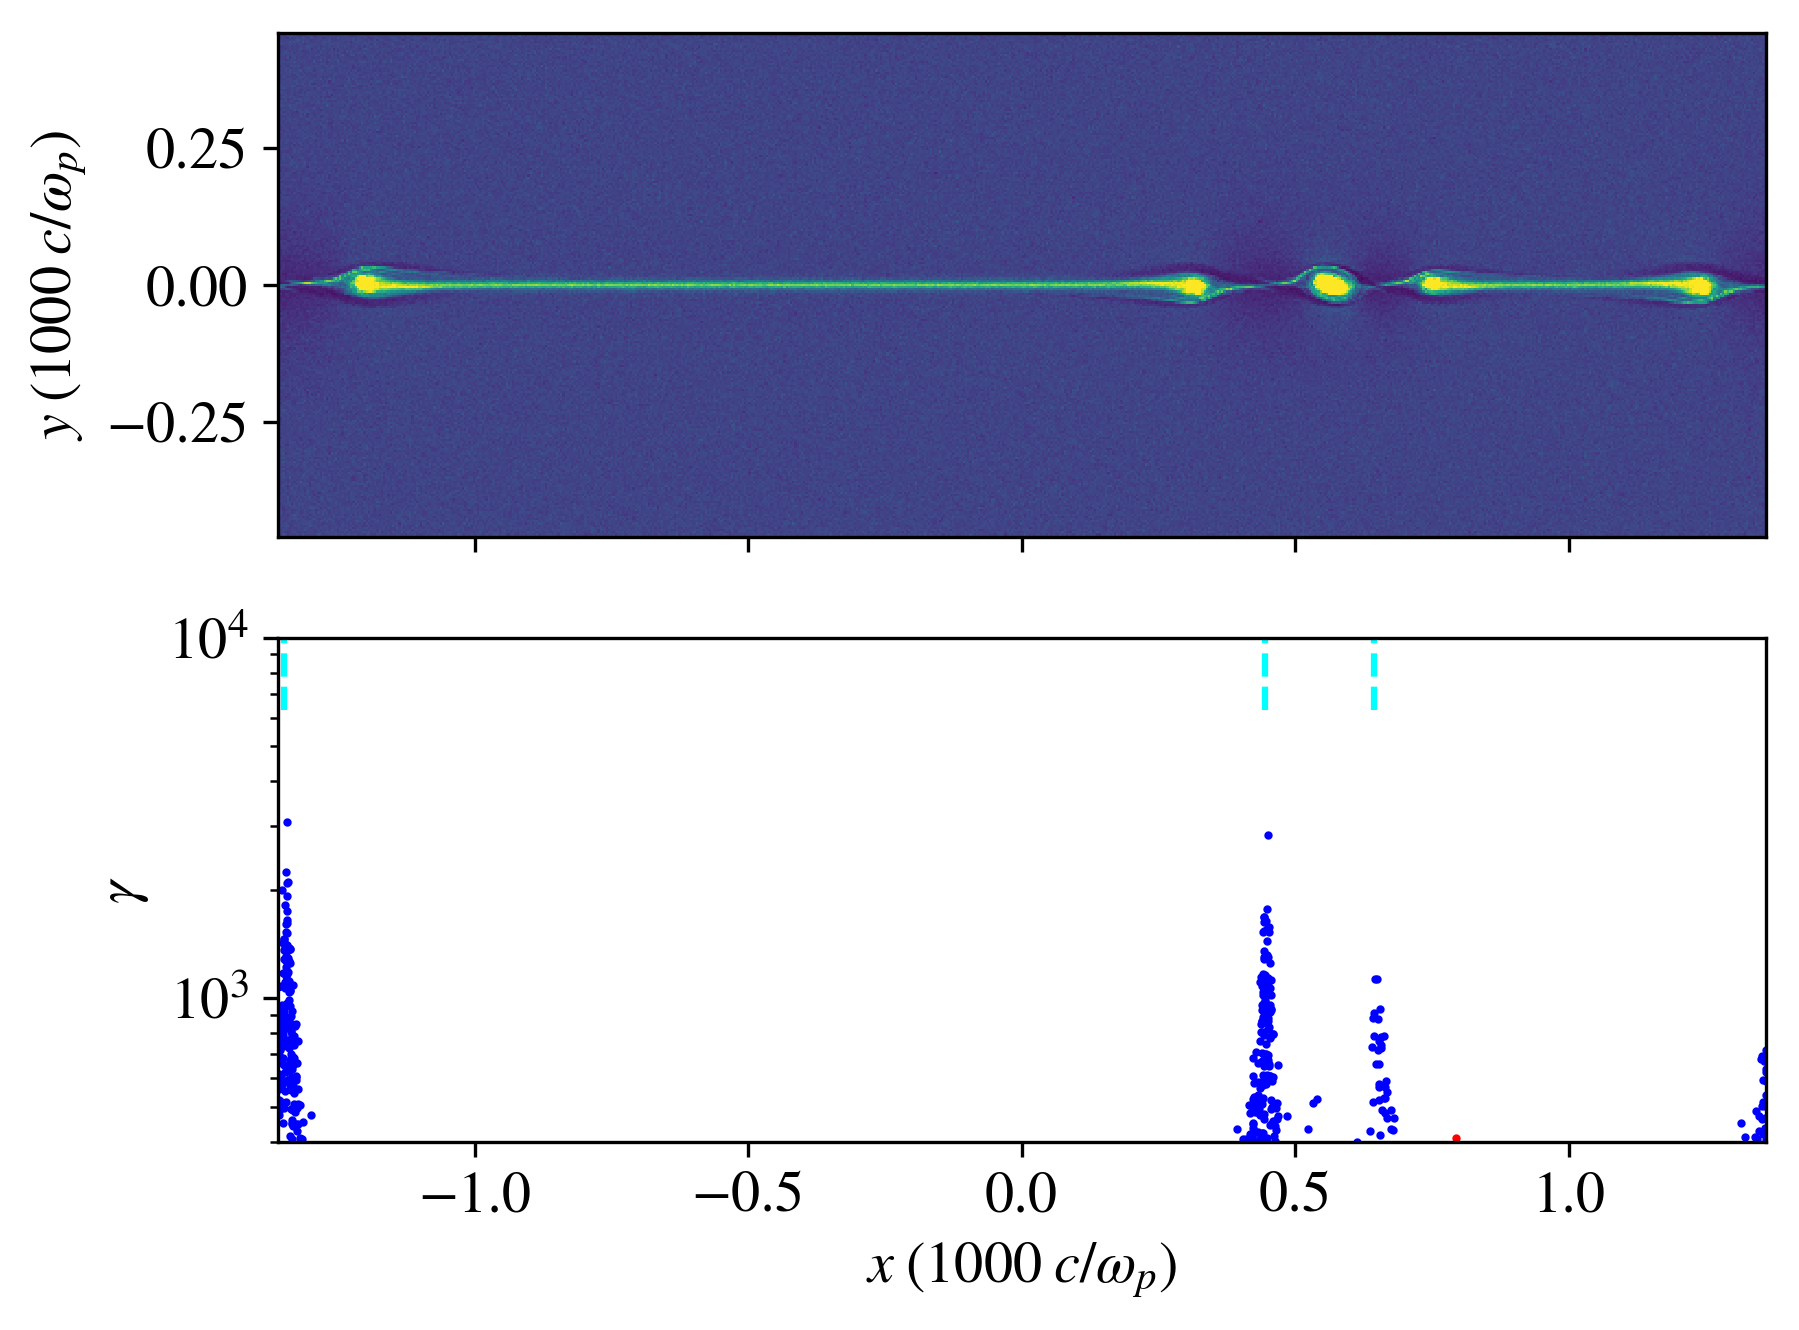
\includegraphics[width=\linewidth]{untriggered_bguide_snapshot7.png}
	}
	\newline
	{
		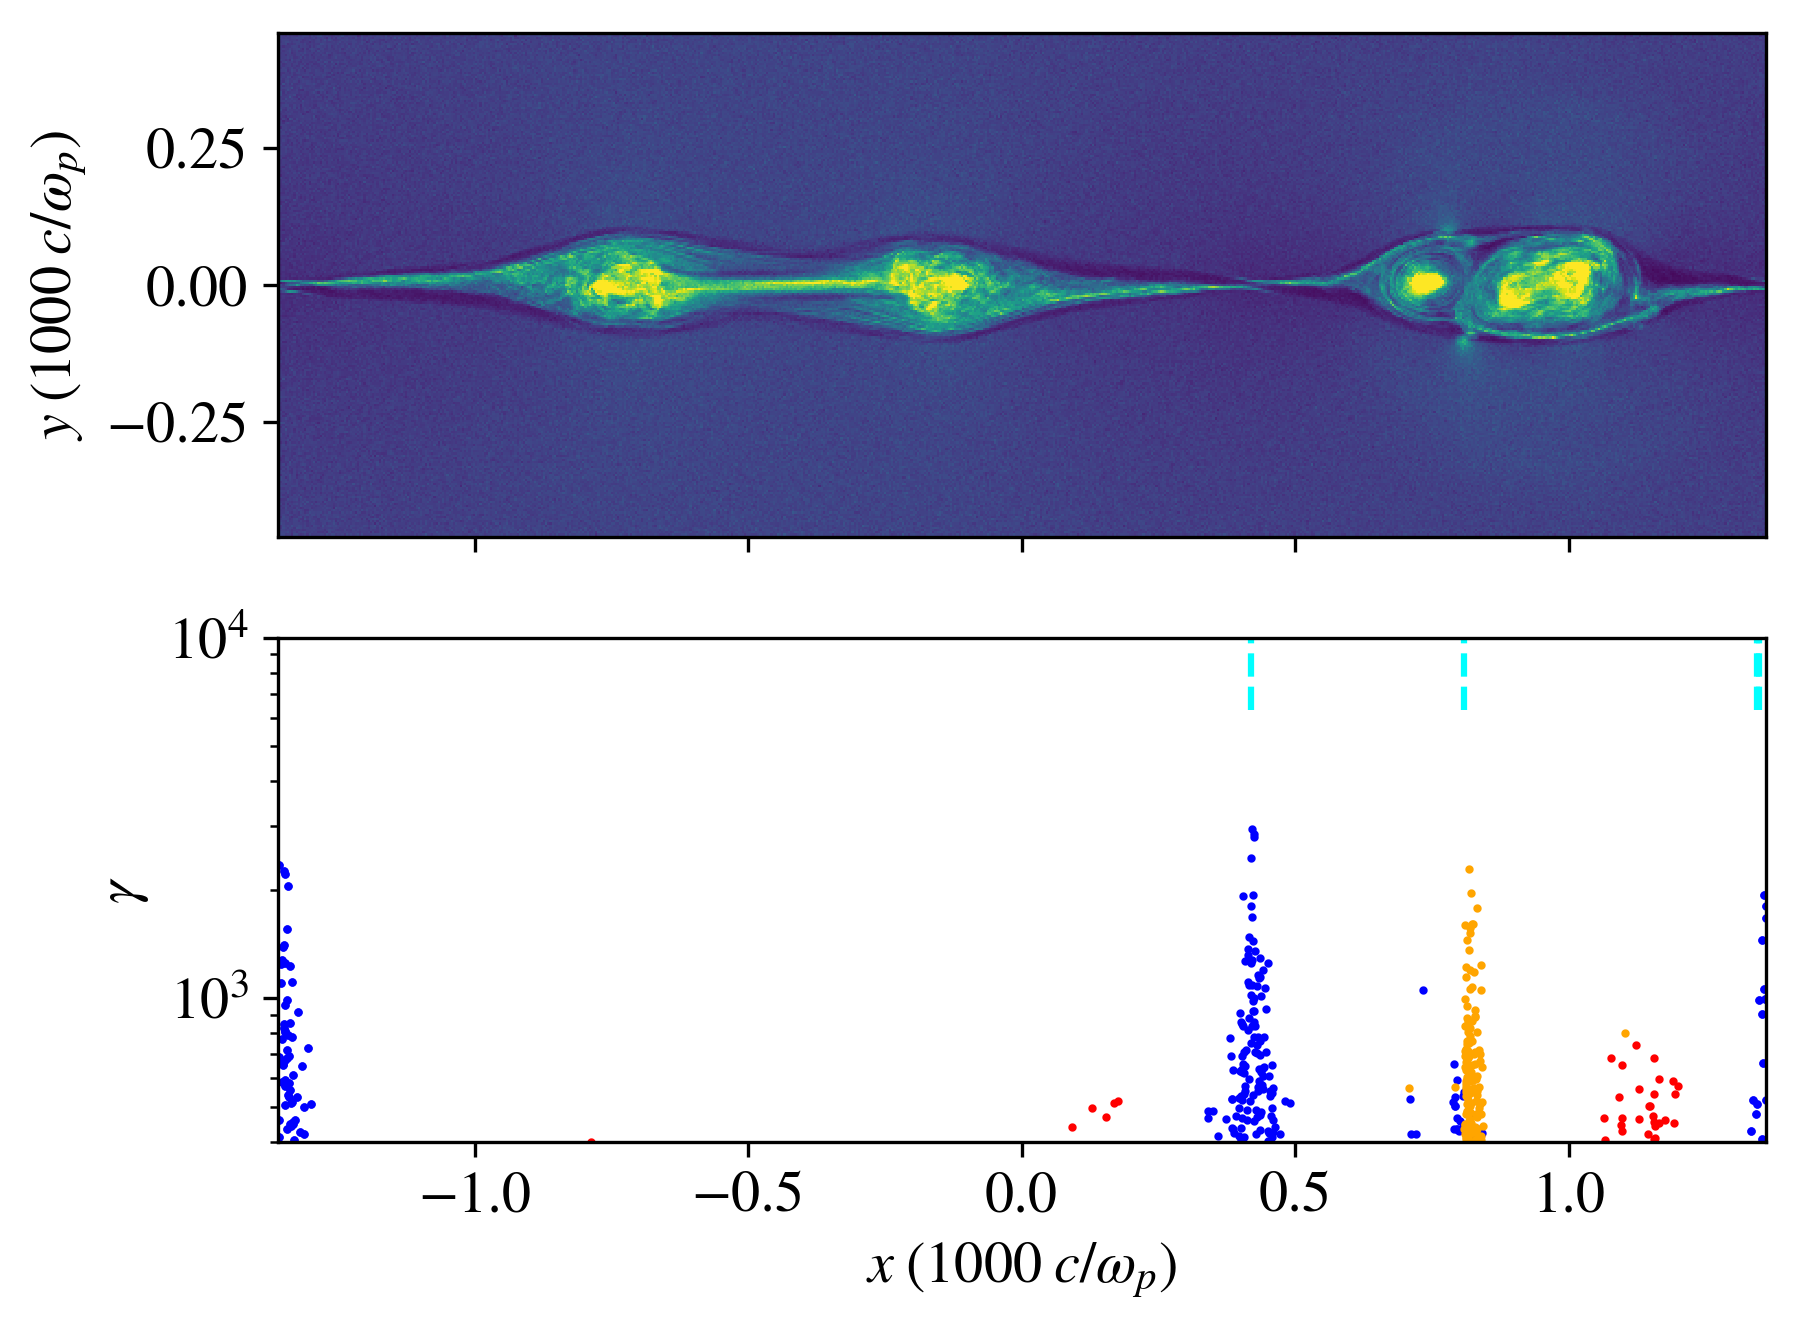
\includegraphics[width=\linewidth]{untriggered_bguide_snapshot12.png}
	}
	\newline
	{
		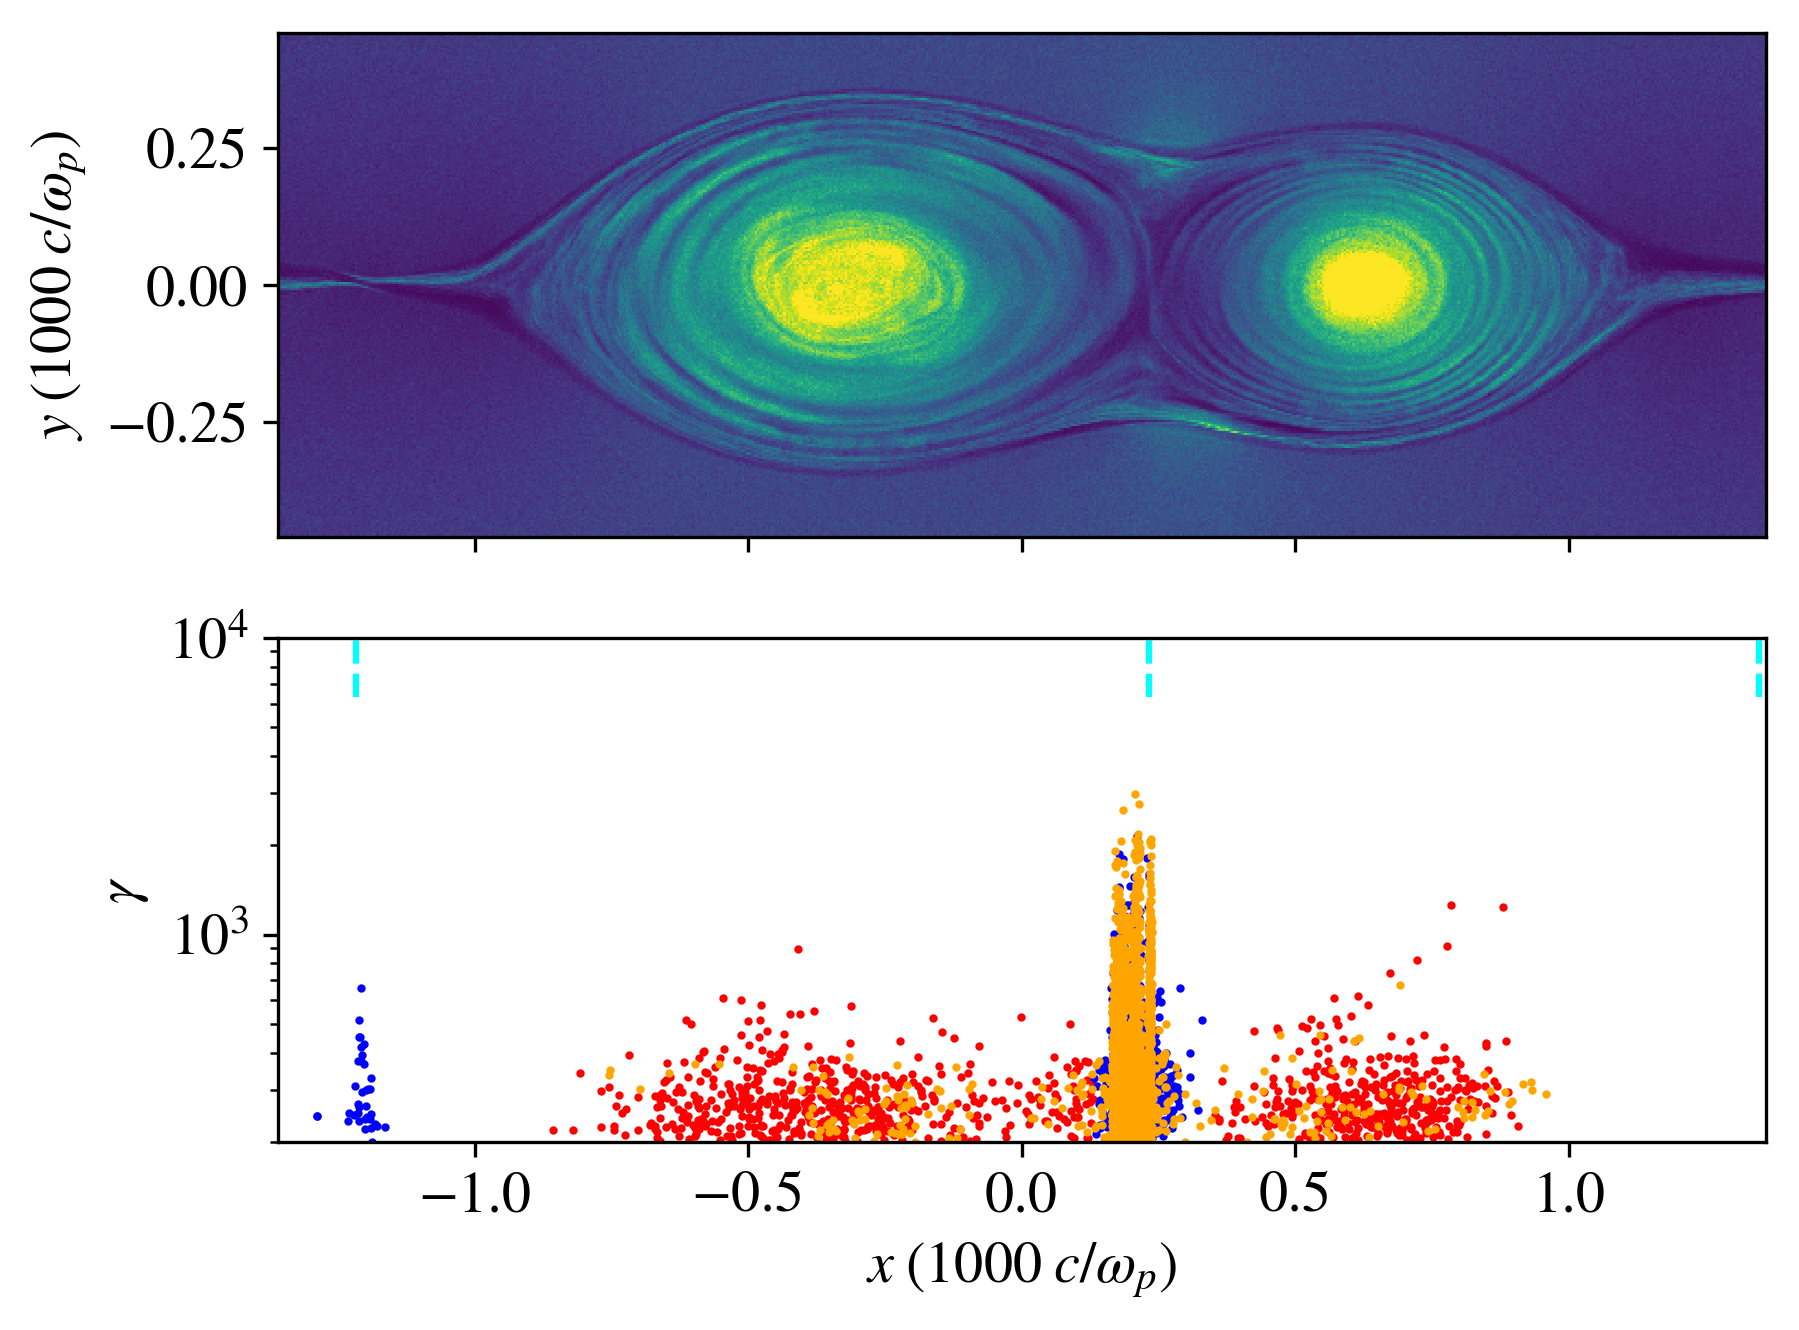
\includegraphics[width=\linewidth]{untriggered_bguide_snapshot45.png}
	}
	
	\caption{Snapshots at three different times from the untriggered simulation with a guide field strength of $B_{g}=0.3B_{0}$.  Because we do not trigger reconnection, numerous primary x-points form and we see numerous primary x-points and plasmoid mergers throughout the simulation domain.
	}
	\label{untriggered_bguide_snapshots}
\end{figure}

\begin{figure}[htp]
	
	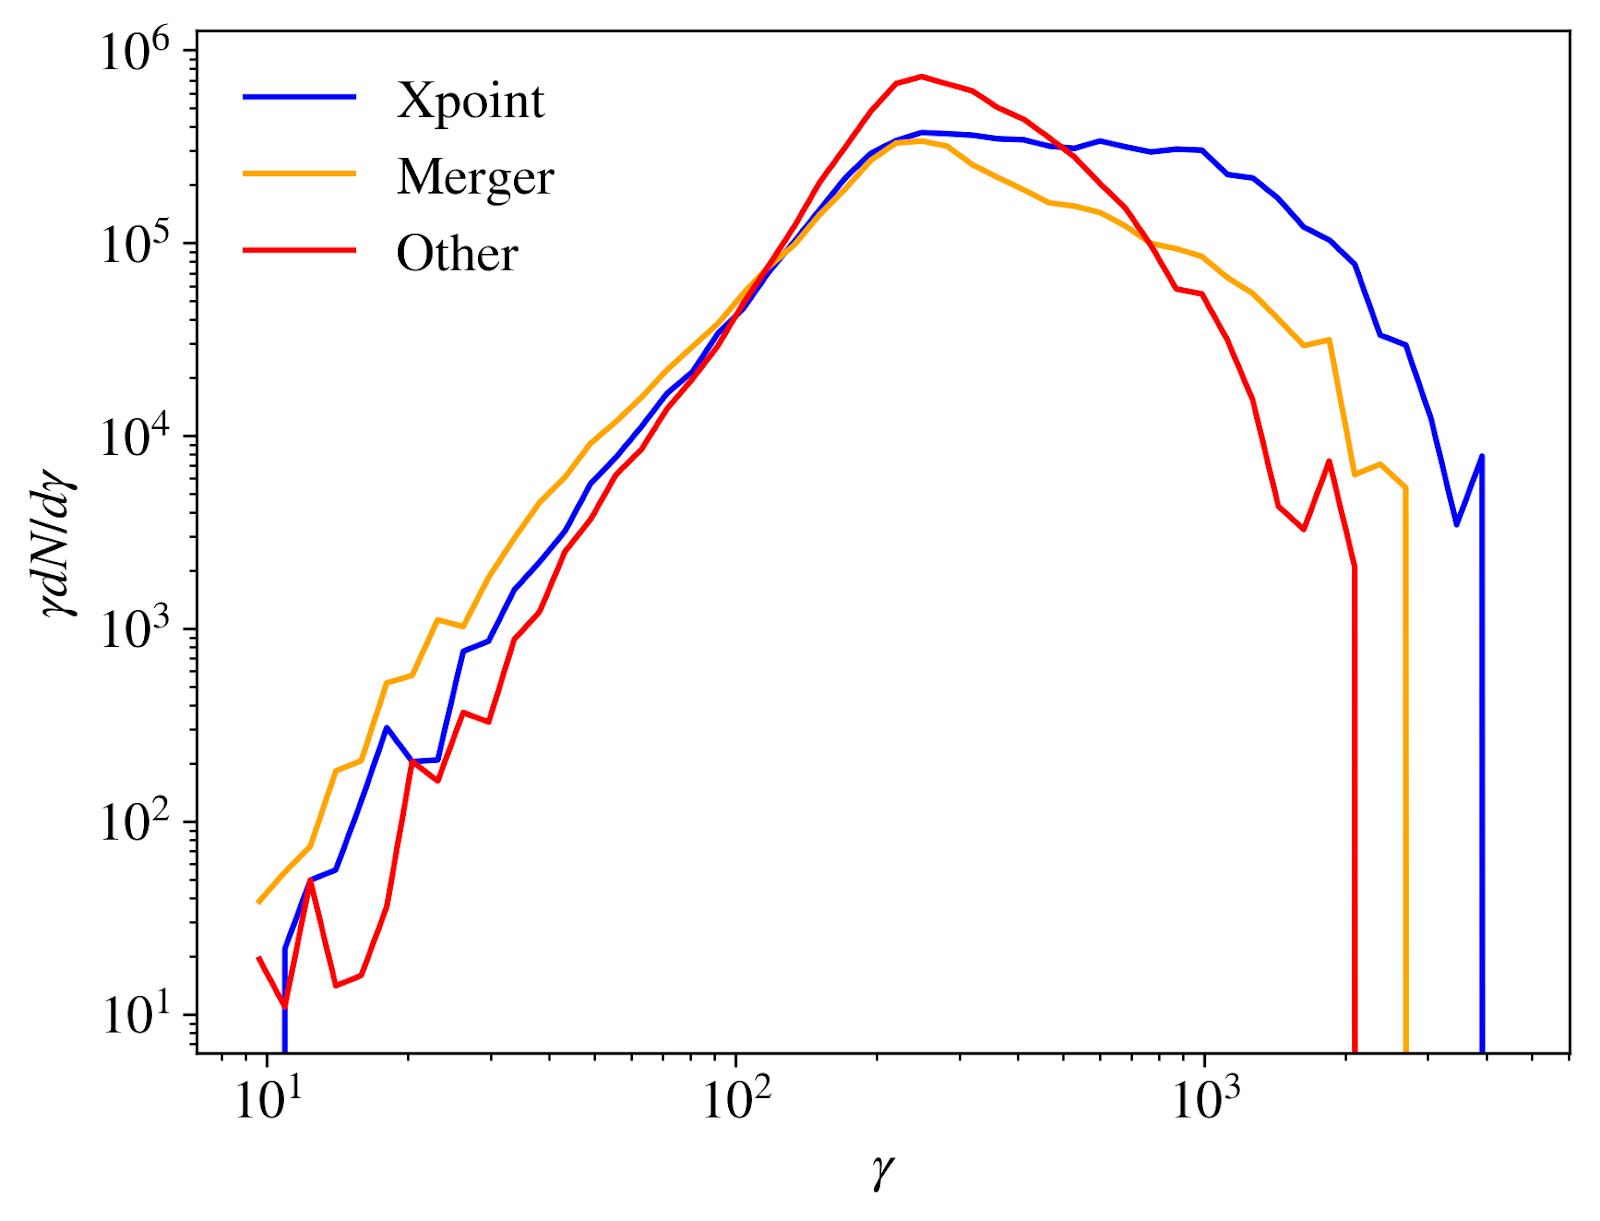
\includegraphics[width=\linewidth]{untriggered_bguide_spec.png}
	\caption{Time-integrated electron spectra from the untriggered simulation with guide field of strength.  While x-points still dominate the highest-energy acceleration episodes, mergers play a much more significant role than in the triggered case (Figures \ref{triggered_bguide_snapshots} and \ref{triggered_bguide_spec}).}
	\label{untriggered_bguide_spec}
\end{figure}

In order to explore the effect of having numerous primary x-points, we show in Figure \ref{untriggered_bguide_snapshots} snapshots from the untriggered simulation with the same guide field strength of $B_{g}=0.3B_{0}$.  At early times (top two panels), we see the primary tearing mode pinch the current sheet at three locations, resulting in three primary x-points, all of which serve as sites of particle acceleration.  In the middle two panels, we see two of the primary plasmoids merging at $x \approx 0.77$, accelerating numerous particles.  In an untriggered setup, such as this one, the primary plasmoids hierarchically merge, resulting in very large plasmoid mergers at late times, which we see in the bottom panels.  As these large plasmoid merge, they accelerate a large number of particles as their magnetic fields reconnect.  

We show the cumulative spectra from this simulation in Figure \ref{untriggered_bguide_spec}.  We see that the x-points are still the dominant source of high-energy particles, but now the mergers also generate a larger number of high-energy particles as compared to the previous triggered simulation.  This is because mergers are inevitable in an untriggered setup, as long as the dominant wavelength of the tearing mode produces numerous primary x-points (and hence, plasmoids) in the given domain.  We note that the contributions to high-energy particle acceleration between x-points and mergers is likely a function of the number of x-points per unit length in the sheet.  As such, the initial thickness of the current sheet in an untriggered setup plays an important role in setting the relative importance of x-points and mergers, and will affect the the overall spectrum of non-thermal particles.  

%move to discussion?
%In some sense, we can think about a triggered simulation as the thick-sheet limit of an untriggered simulation, where the dominant wavelength of the tearing mode is comparable to the system size, and hence only generates a single x-point.  We also note that in the limit of large domains, we will still have the same number of x-points per unit length, set by the dominant wavelength of the primary tearing mode.  Because of this, we expect that the spectra will be much less sensitive to the size of the domain than in the triggered setup, where only one x-point is present, and hence the number of x-points per unit length decreases as $\sim 1/L$.



\begin{figure}[htp]
	{
		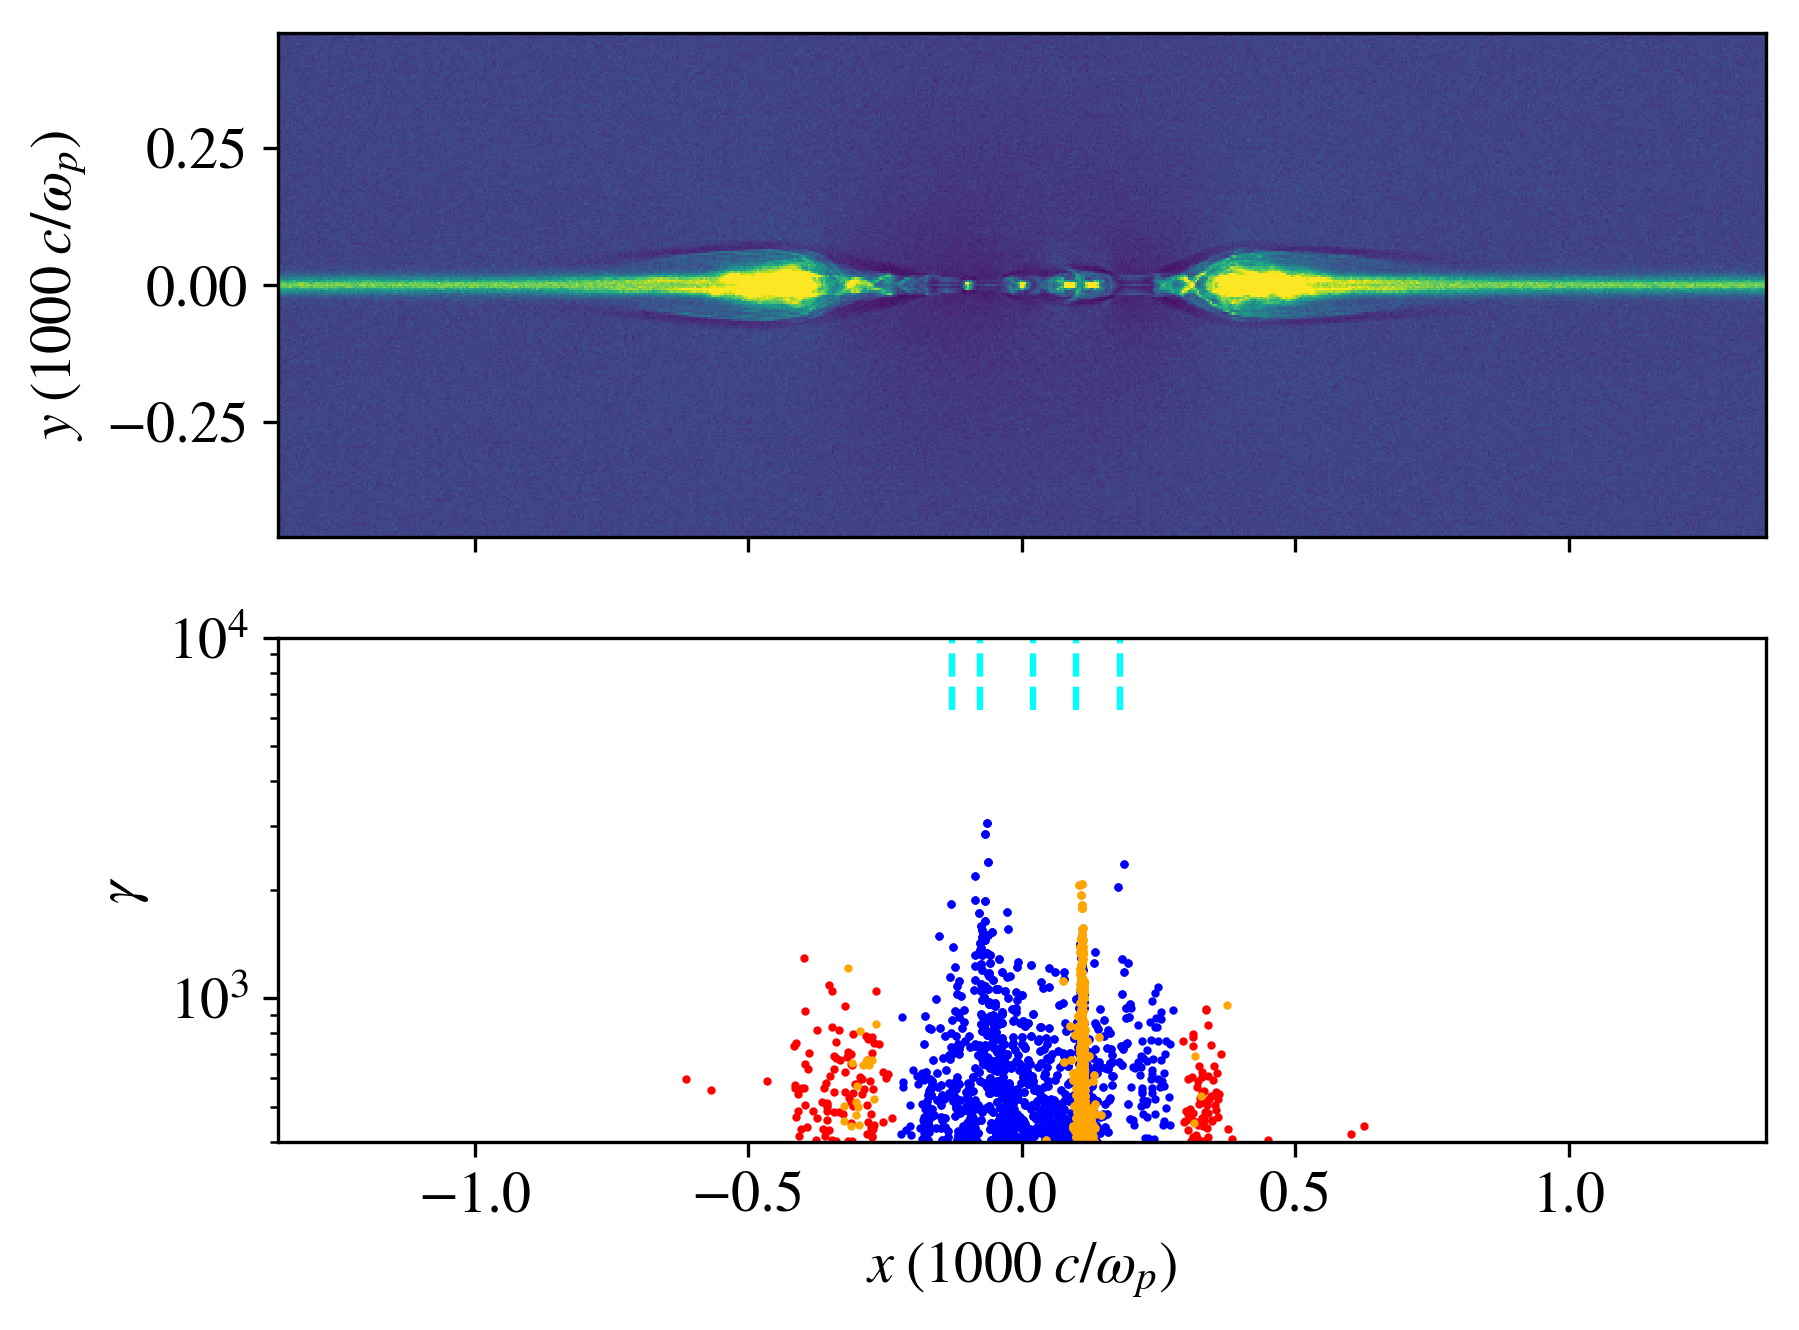
\includegraphics[width=\linewidth]{triggered_bguide0_snapshot8.png}
	}
	\newline
	{
		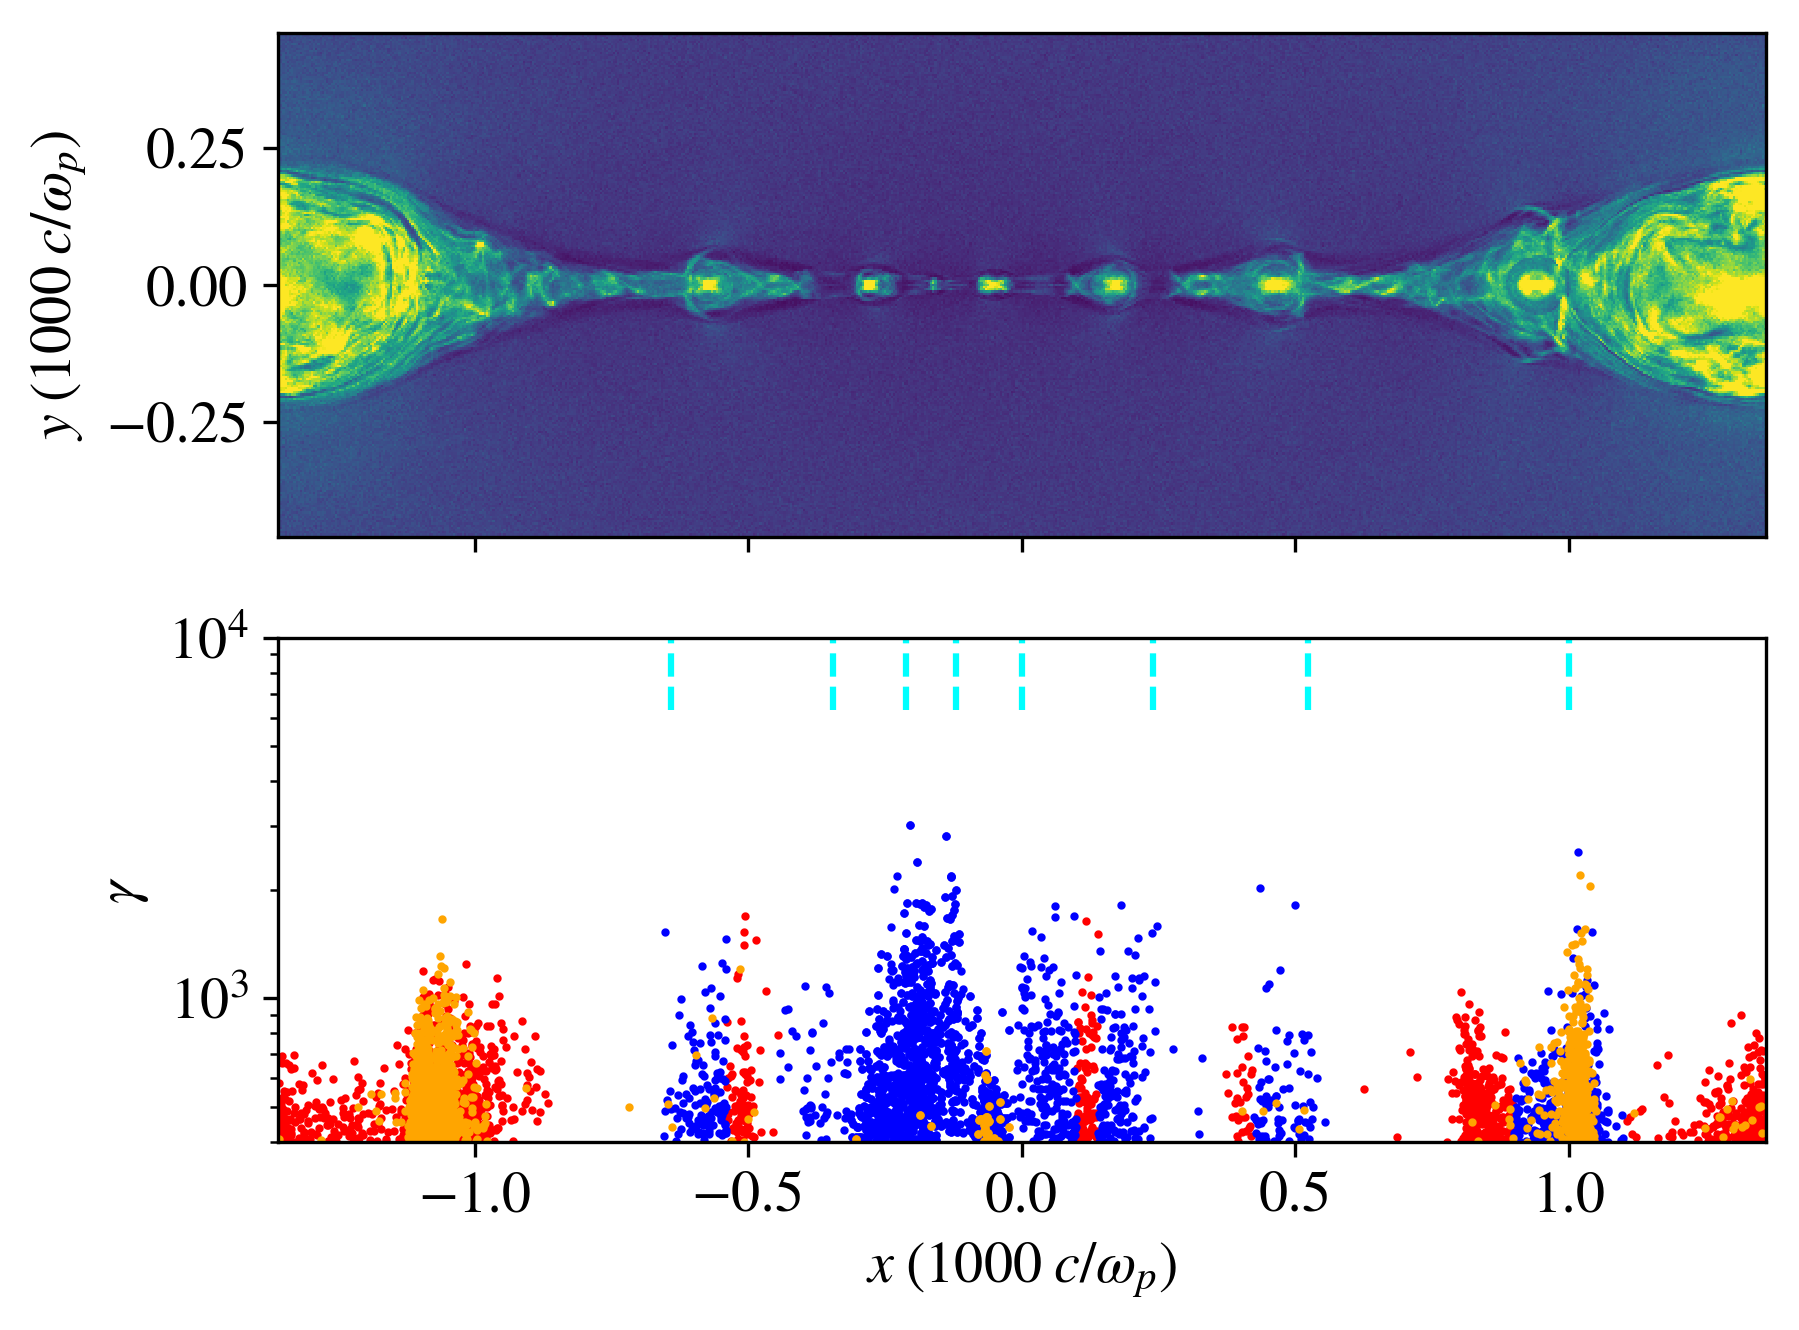
\includegraphics[width=\linewidth]{triggered_bguide0_snapshot18.png}
	}
	\newline
	{
		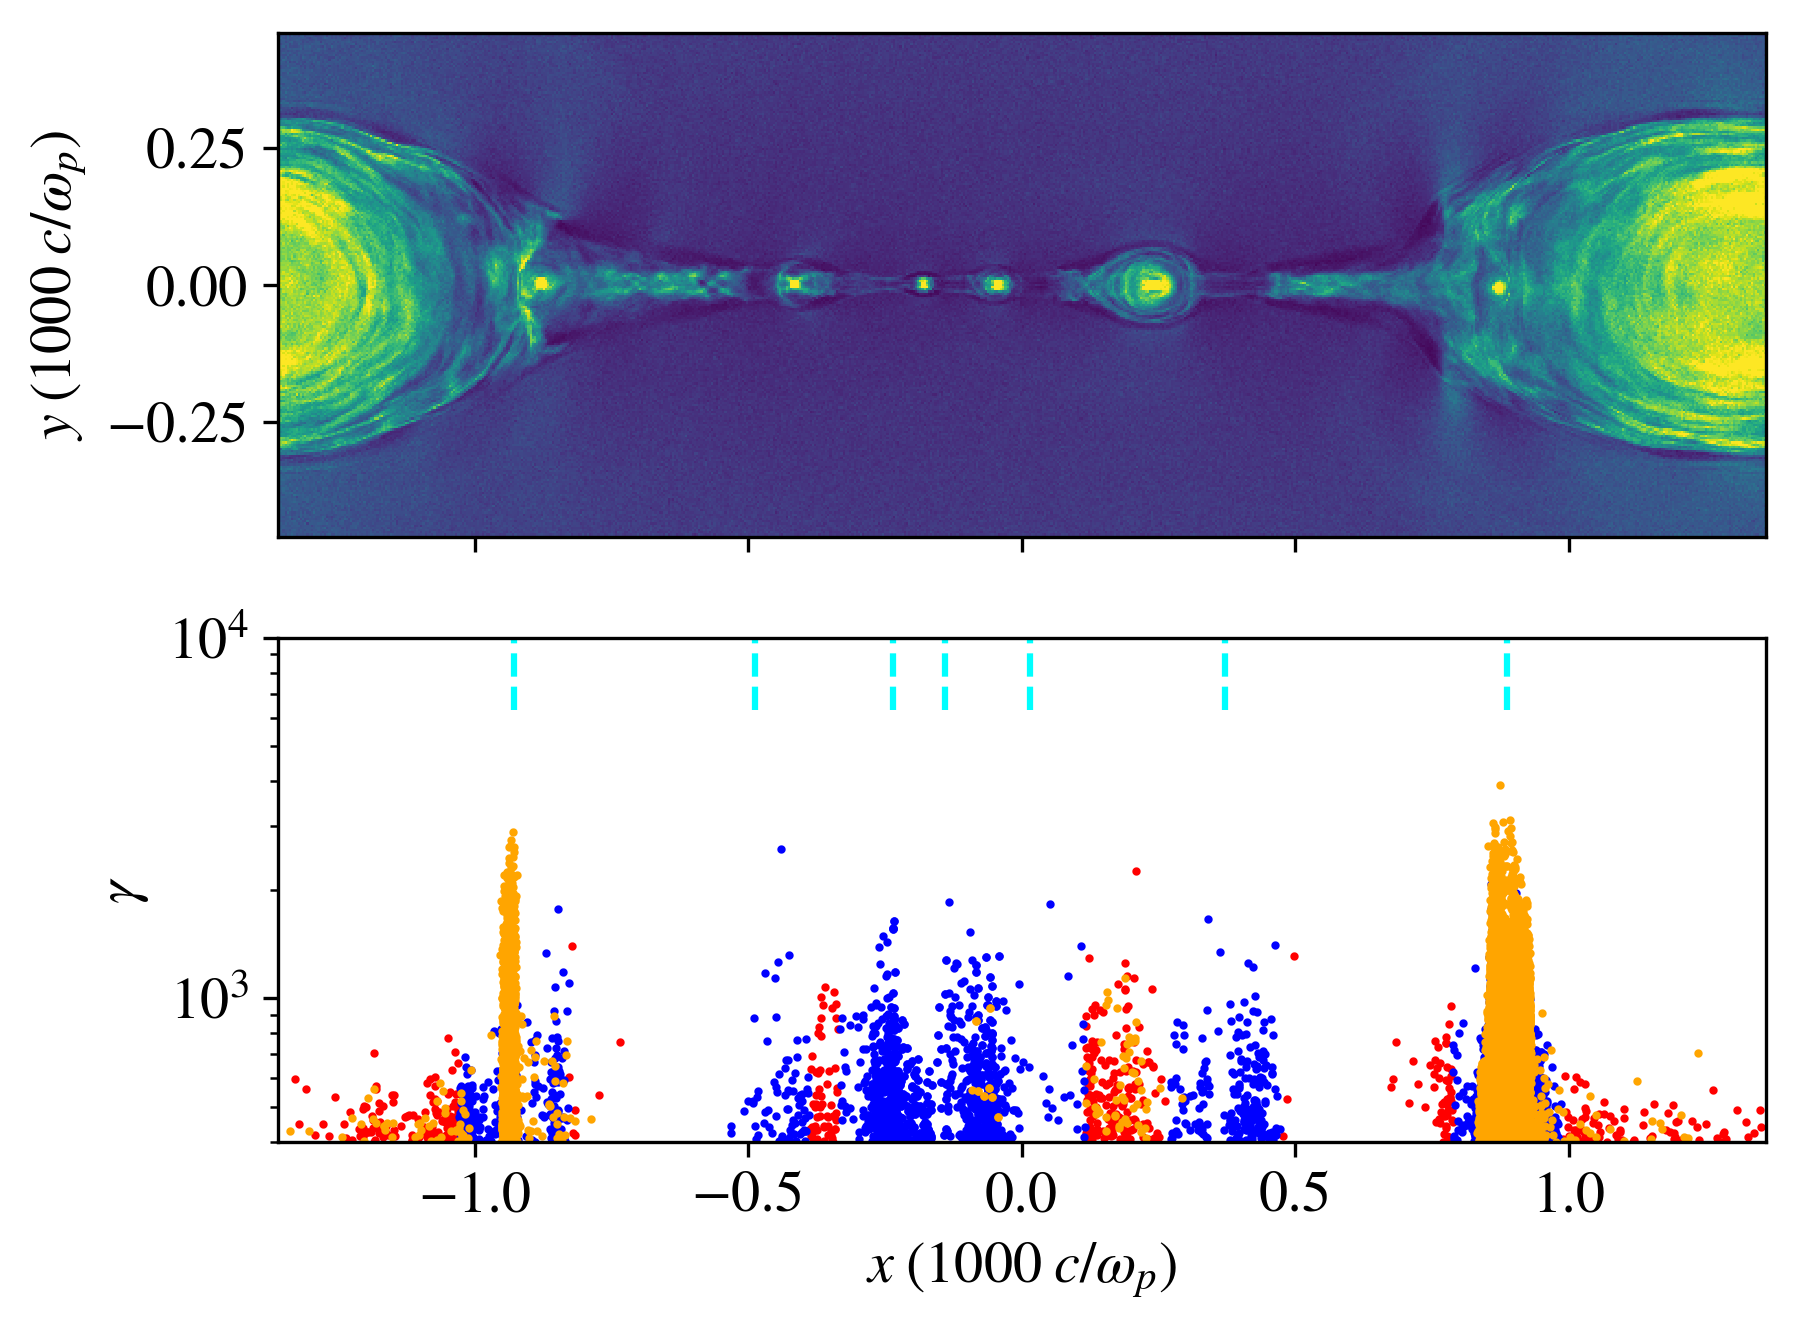
\includegraphics[width=\linewidth]{triggered_bguide0_snapshot25.png}
	}
	
	\caption{Snapshots at three different times from the untriggered simulation with no guide field.  The secondary tearing mode fractures the current sheet throughout the domain, resulting in numerous x-points and secondary plasmoids.  
	}
	\label{triggered_bguide0_snapshots}
\end{figure}

We show in Figure \ref{triggered_bguide0_snapshots} three snapshots from the triggered simulation with no guide field.  We see at early times that numerous closely-spaced secondary x-points have already formed in the region vacated by the reconnection fronts.  Two small plasmoids at $x\approx 0.1$ are merging.  Due to the prevalence of the secondary tearing mode and associated plasmoid mergers, acceleration is not as localized as in the previous cases with a guide field.  This trend continues in the middle panel, where secondary x-points are accelerating particles all throughout the central $\sim 1/3$ of the domain.  The secondary plasmoids that form are inevitably pulled towards the edge of the domain, ultimately merging with the large boundary island, accelerating particles in merging events.  This trend continues to later times (bottom panels): acceleration at secondary x-points and the associated merging of secondary plasmoids remains active until the magnetic island at the boundary grows so large that it chokes off the inflowing plasma and reconnection halts.  

When we compare the relative contributions of x-points and mergers to the electron energy spectrum, in Figure \ref{triggered_bguide0_spec}, we find that both x-points and mergers accelerate a large number of particles above $\gamma=1000$.  Mergers slightly dominate over x-points in overall number of particles that are accelerated to these highly relativistic energies.


\begin{figure}[htp]
	
	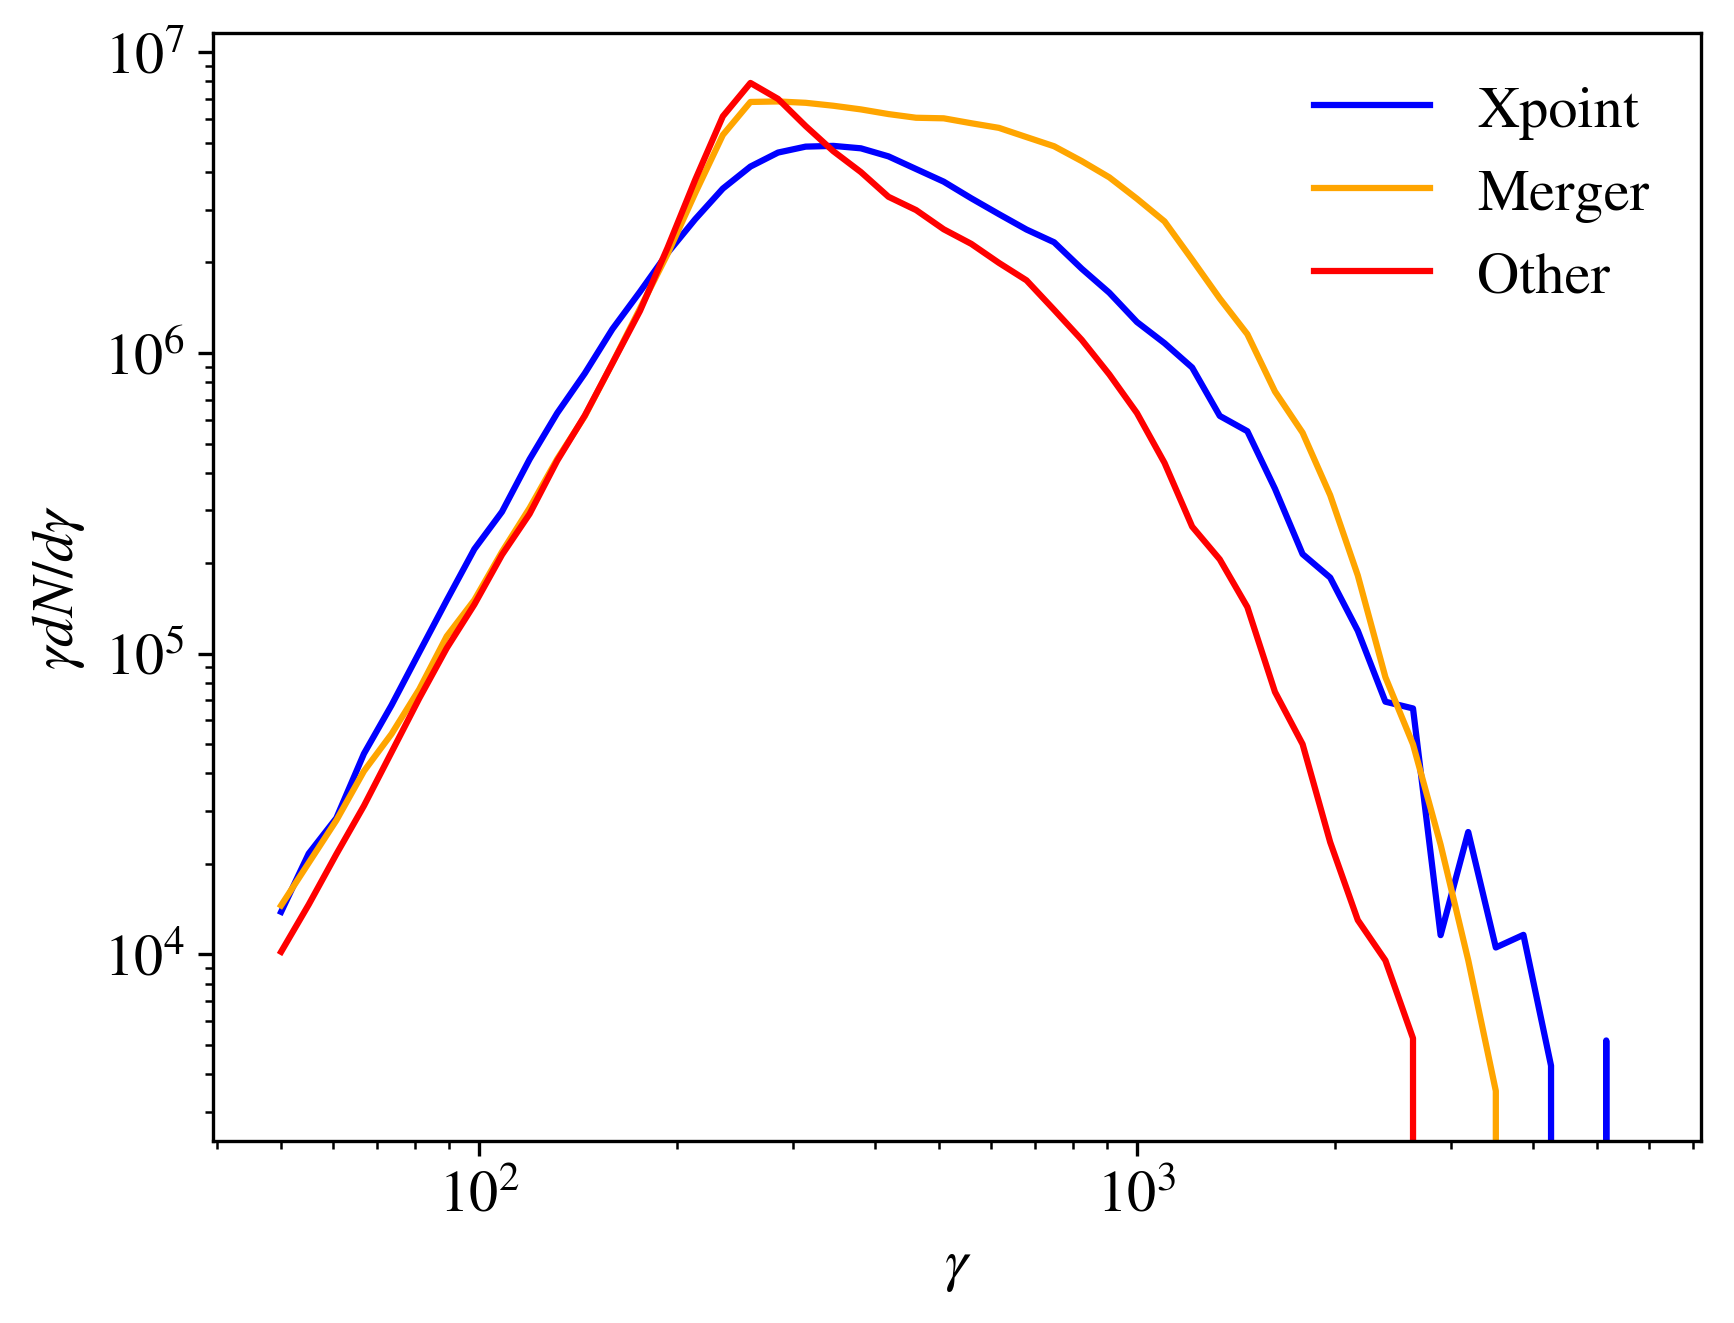
\includegraphics[width=\linewidth]{8k_bguide0_triggered_accmec_spect.png}
	\caption{Time-integrated electron spectra from the triggered simulation with no guide field.  We see that the copious production of secondary plasmoids leads to mergers dominating over x-points for high-energy acceleration.}
	\label{triggered_bguide0_spec}
\end{figure}

We finally explore the case of an untriggered simulation with no guide field.  We show in Figure \ref{untriggered_bguide0_snapshots} three snapshots from this simulation.  At early times (top panel), numerous primary and x-points quickly form and begin accelerating particles all throughout the domain.  These primary and secondary plasmoids hierarchically merge until the largest plasmoids in the domain merge (middle panel).  Once the largest plasmoid is formed (bottom panel), the secondary tearing mode remains active, producing numerous secondary x-points and plasmoids throughout the domain.  We show in Figure \ref{untriggered_bguide0_spec} the cumulative electron spectra broken down into components.  We see again that both x-points and mergers produce large numbers of high-energy electrons, with mergers being slightly more dominant.

\begin{figure}[!h]
	{
		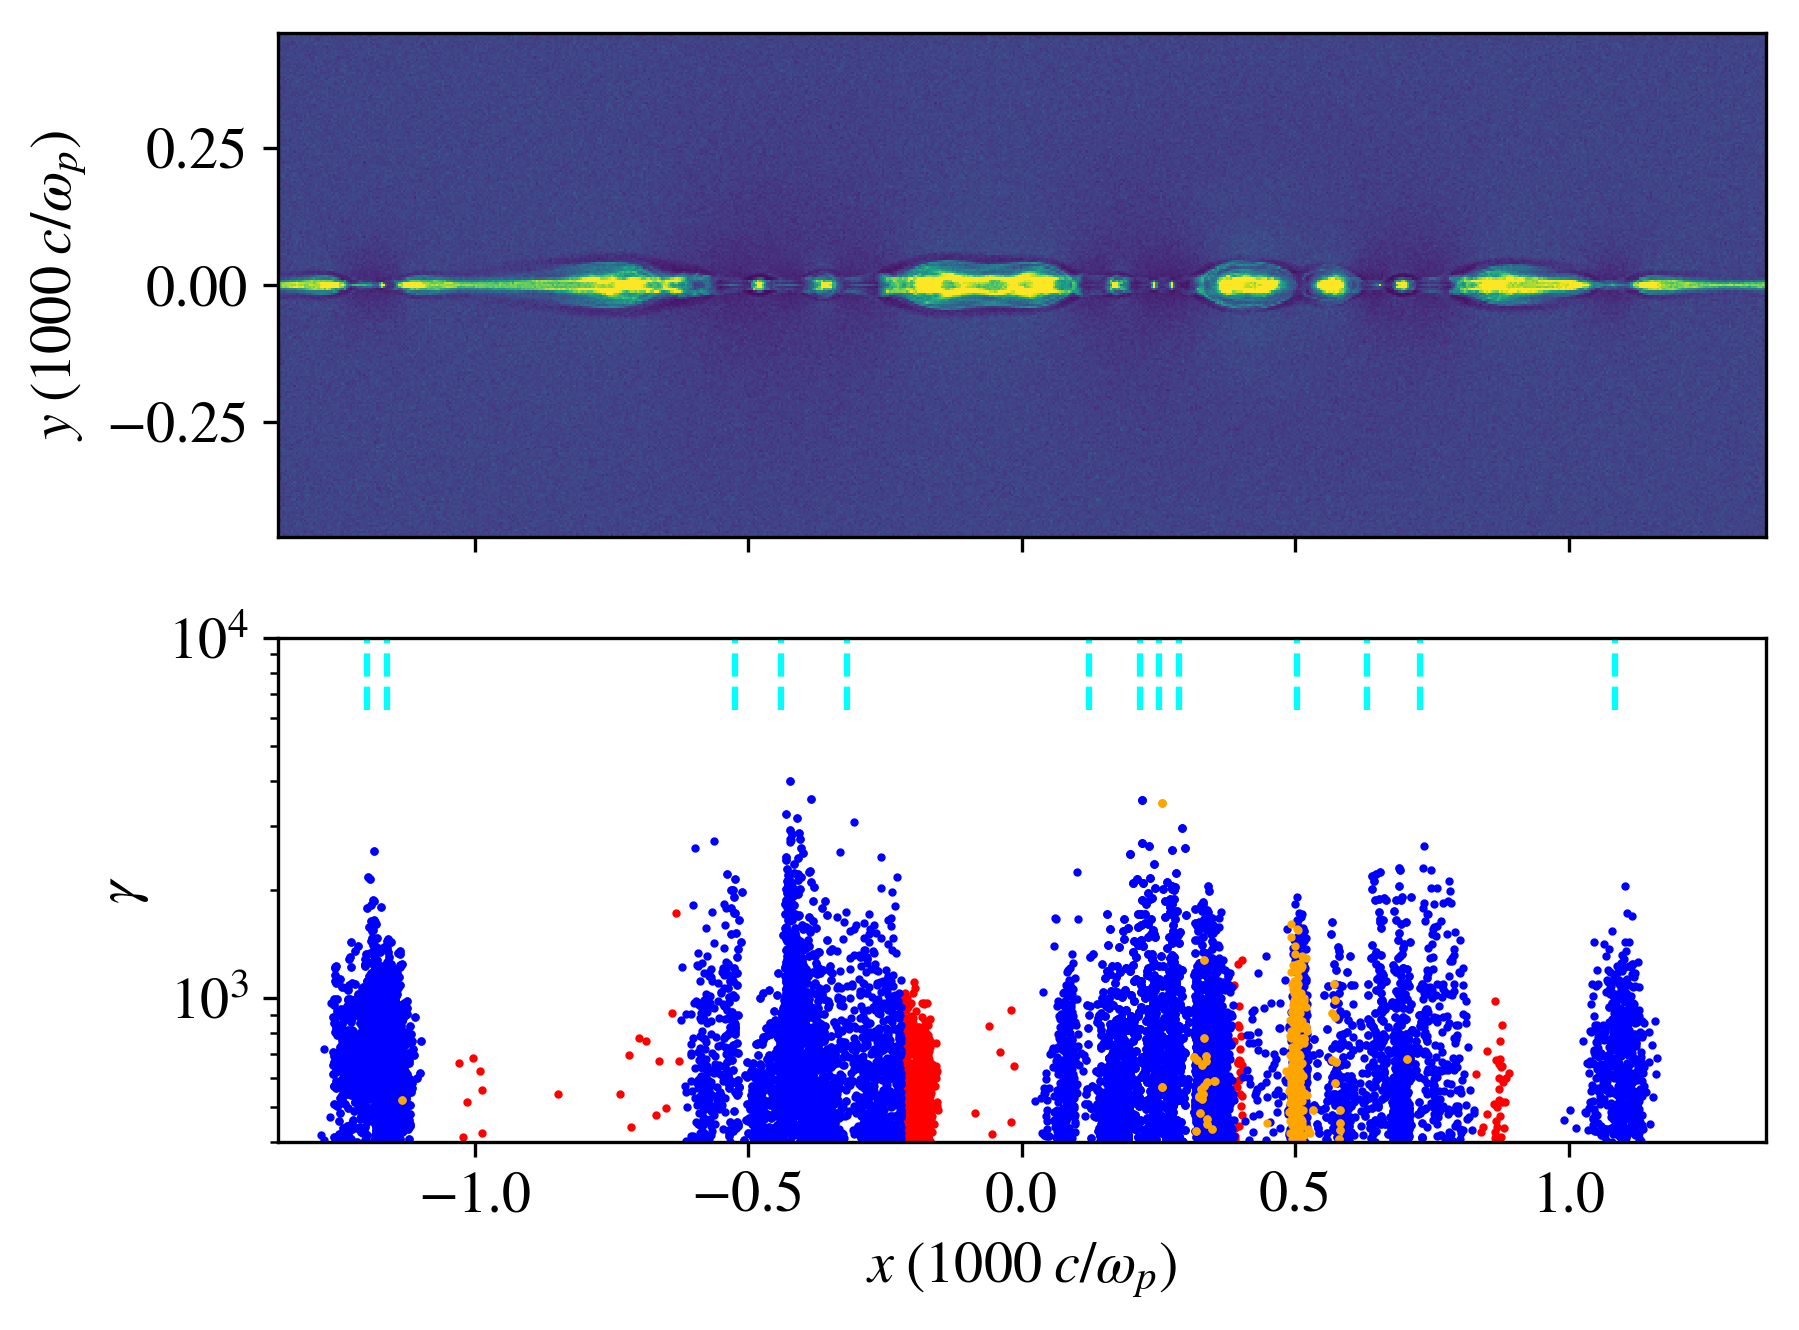
\includegraphics[width=\linewidth]{untriggered_bguide0_snapshot8.png}
	}
	\newline
	{
		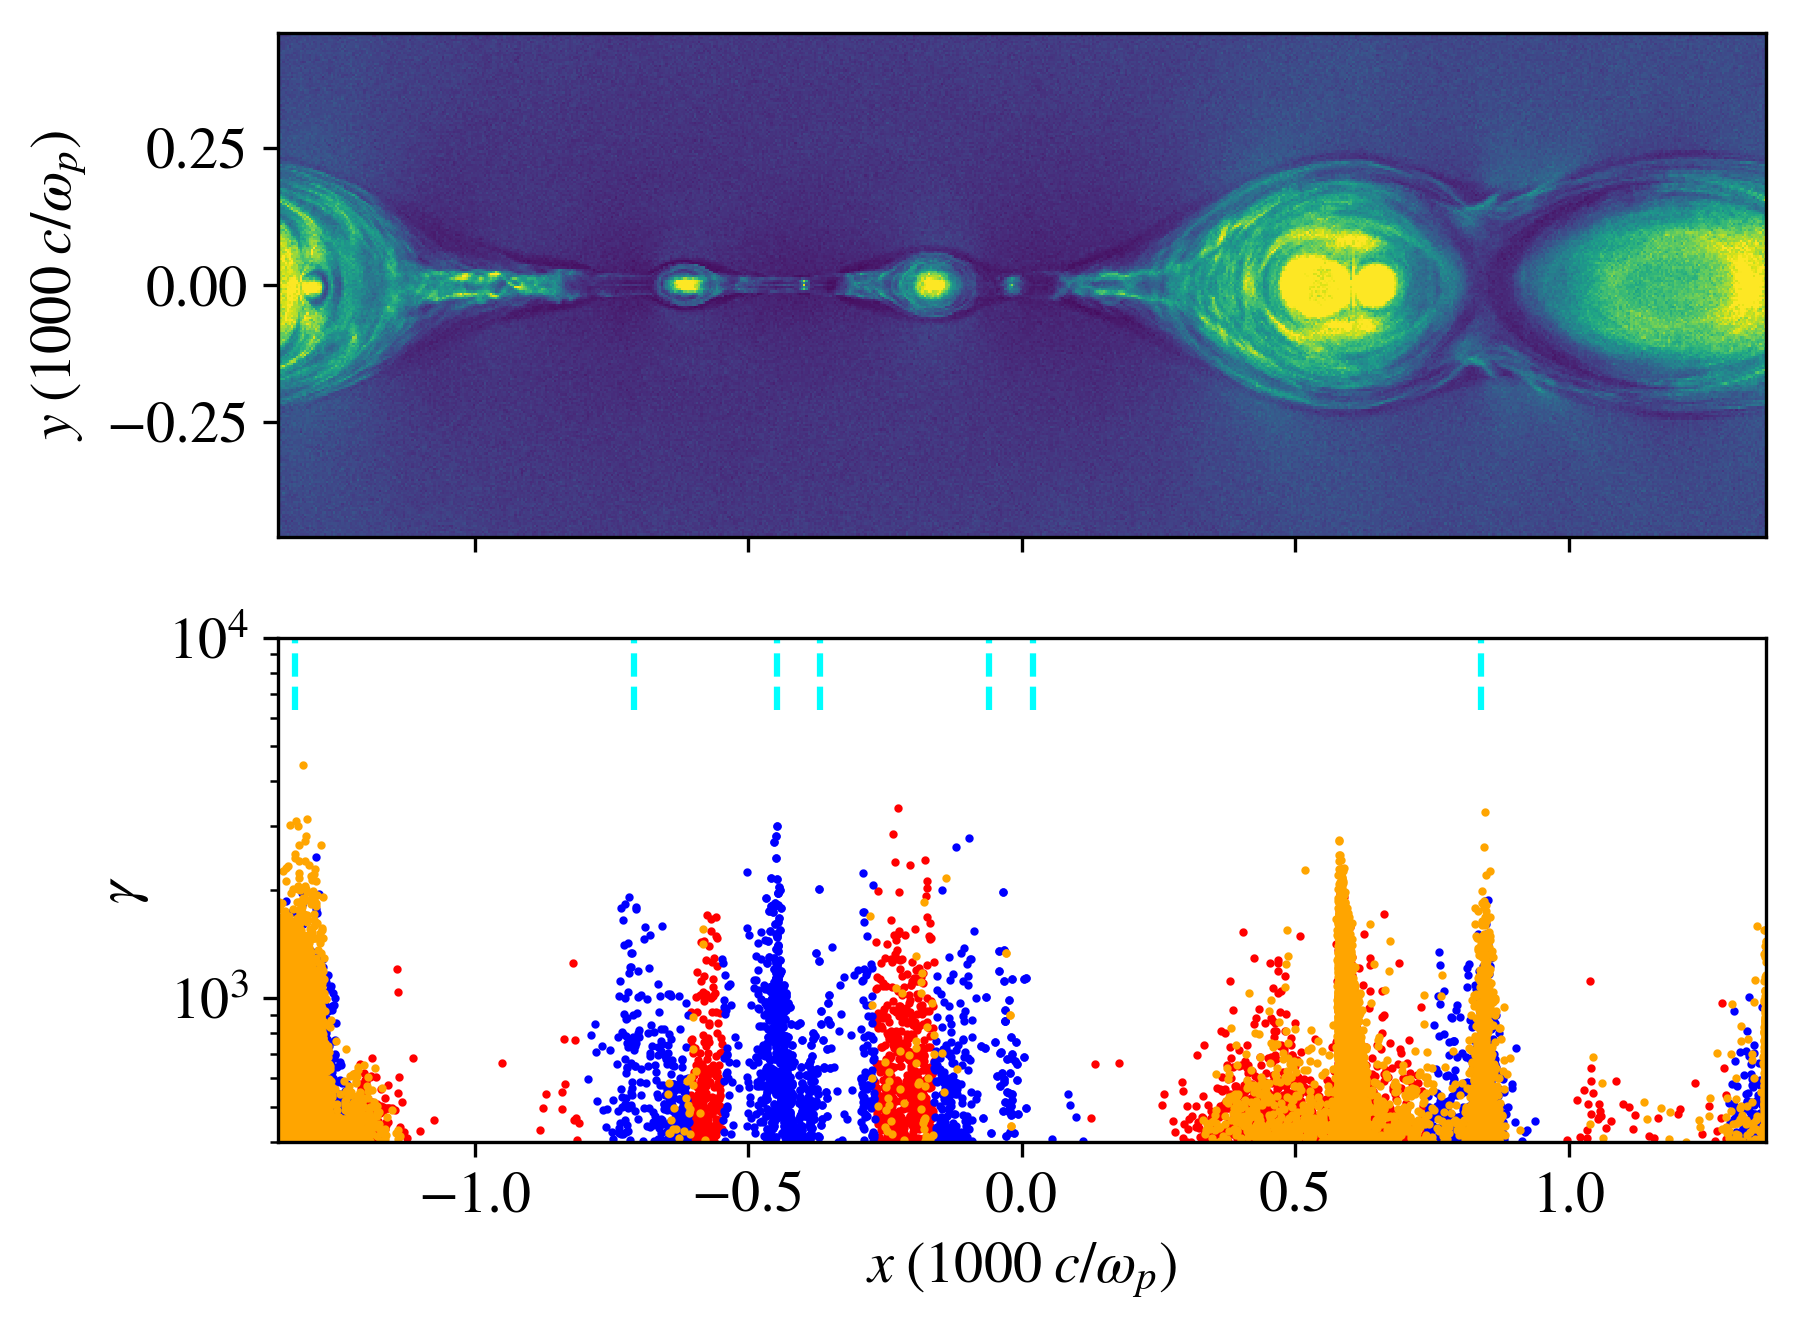
\includegraphics[width=\linewidth]{untriggered_bguide0_snapshot25.png}
	}
	\newline
	{
		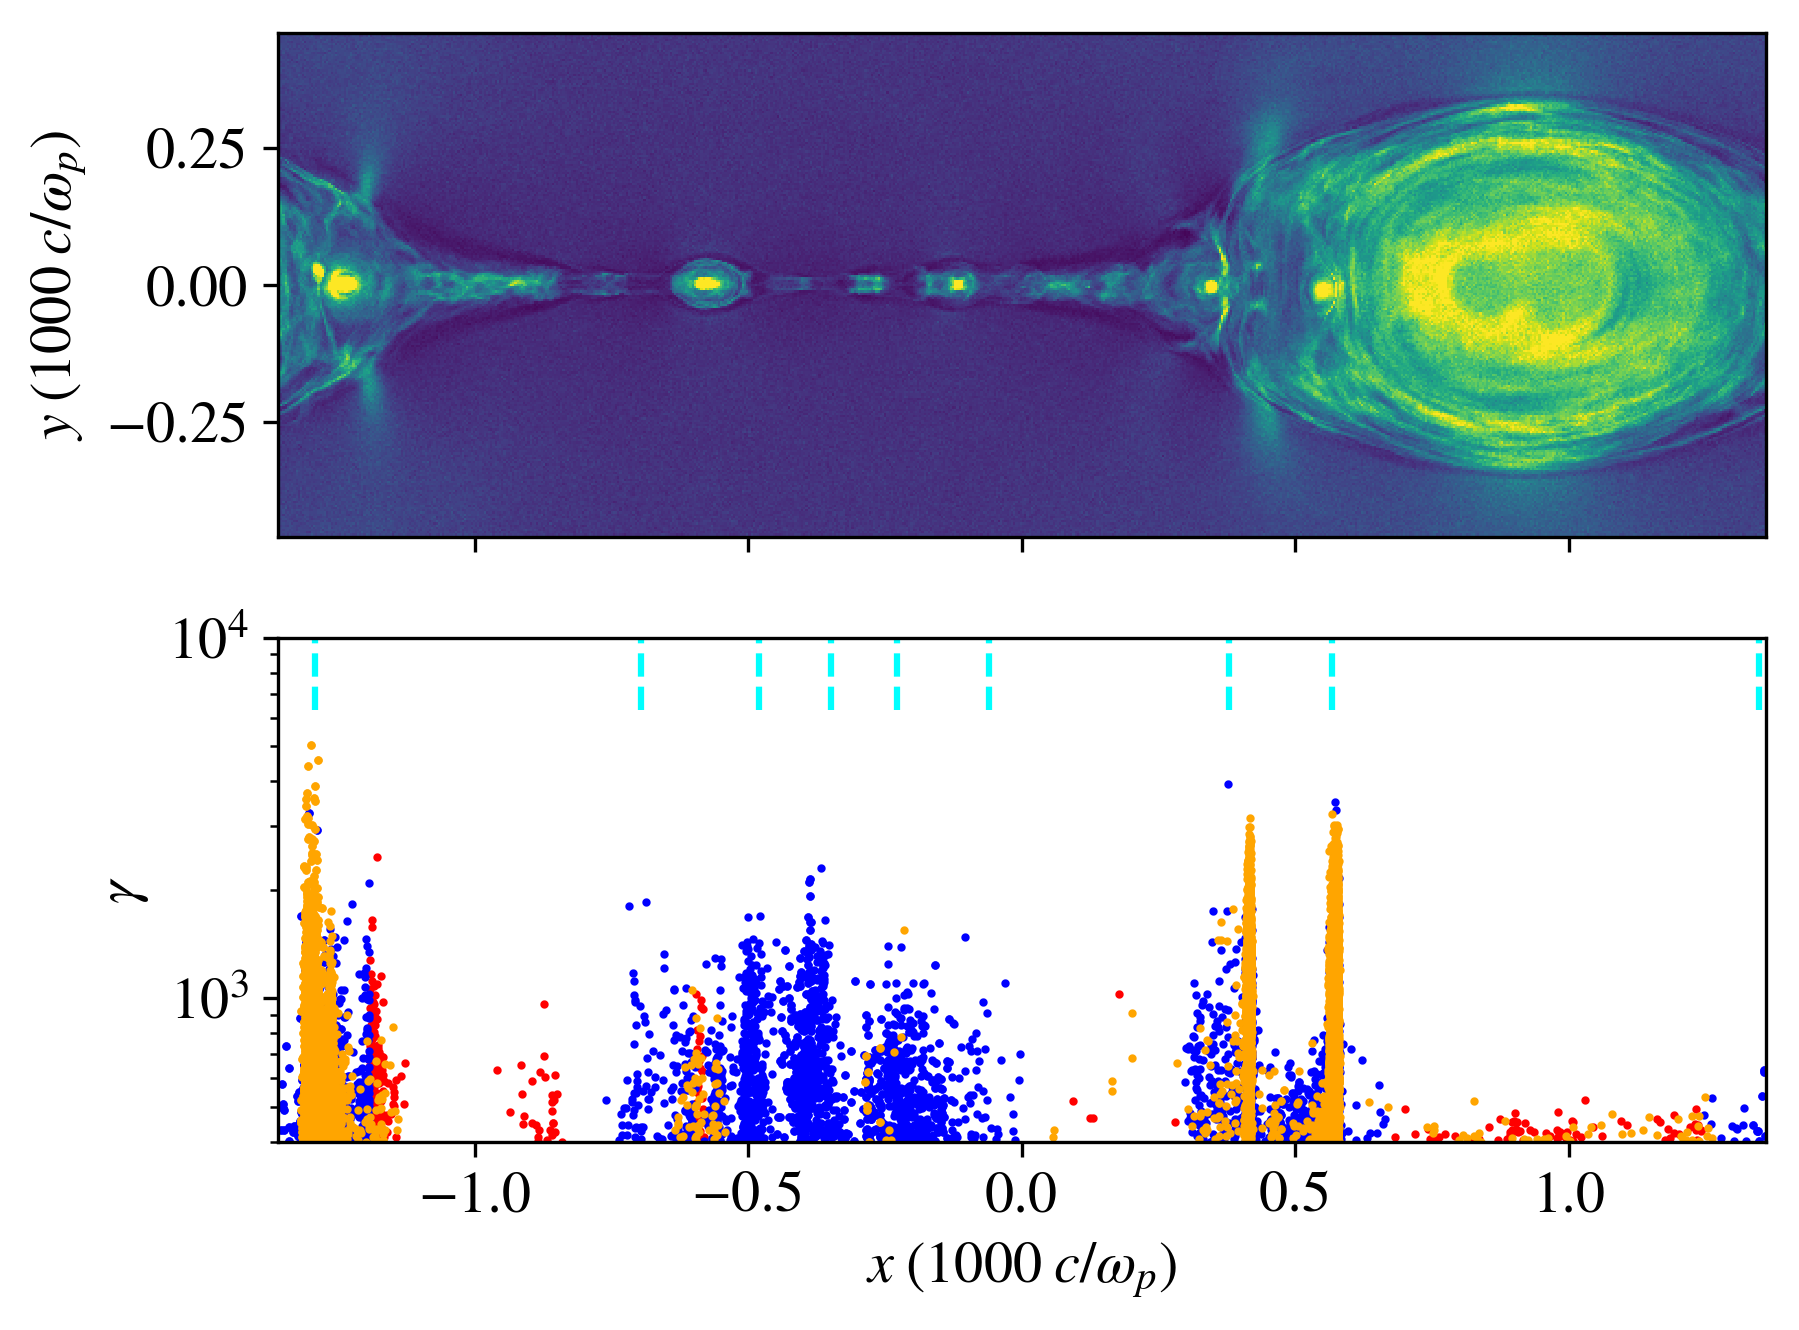
\includegraphics[width=\linewidth]{untriggered_bguide0_snapshot35.png}
	}
	
	\caption{Snapshots at three different times from the untriggered simulation with no guide field.  We see that both the primary and secondary tearing mode result in copious x-point and plasmoid formation and the corresponding electron acceleration.  
	}
	\label{untriggered_bguide0_snapshots}
\end{figure}

\begin{figure}[htp]
	
	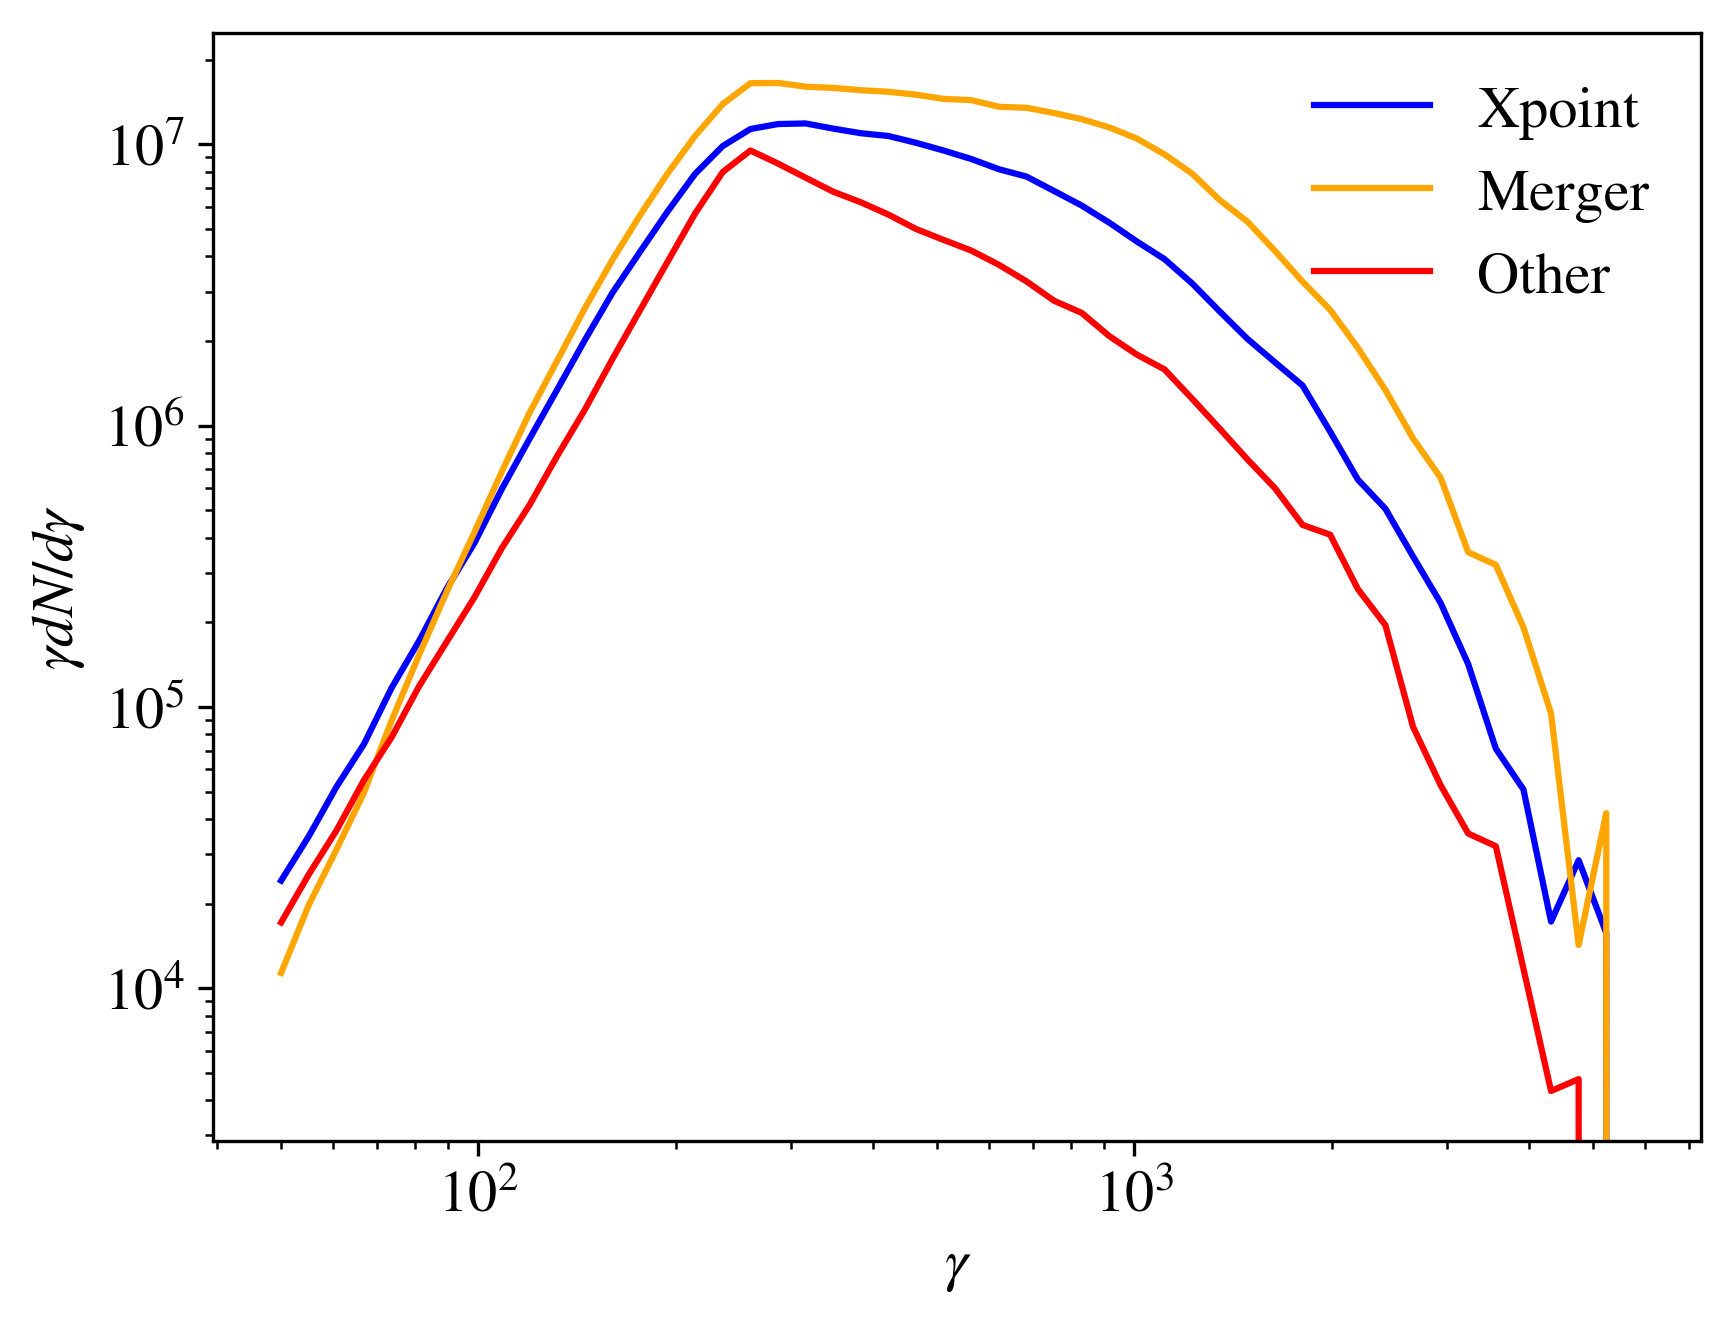
\includegraphics[width=\linewidth]{8k_bguide0_untriggered_accmec_spect.png}
	\caption{Time-integrated electron spectra from the untriggered simulation with no guide field.  The prevalence of plasmoids (both primary and secondary), and their merging results in plasmoid mergers dominating over x-points for high-energy acceleration.}
	\label{untriggered_bguide0_spec}
\end{figure}


%\section{Electron Trajectories}
%In addition to exploring the locations where electrons are first accelerated, we also decompose the work done on the particles into components parallel and perpendicular to the local magnetic field.  This is yet another diagnostic to investigate the relative role of x-points.  As previously discussed, the electric field associated with reconnection at an x-point will be in the $+ \; (-) \;\hat{z}$  direction at an x-point (plasmoid merger).  In the presence of a guide field, this manifests as a nonzero $\vec{E} \cdot \vec{B}$, which will result in acceleration of particles in the direction of the magnetic field.  The work done by electric fields that are perpendicular to the local magnetic field can be understood as the product of the total drift velocity (from, e.g., curvature or $\nabla B$ drifts) dotted into the electric field.  

%Over a particle's trajectory, the change in its kinetic energy is
%\begin{equation}
%W = \int_{t_{0}}^{t_{f}}{q\vec{v}\cdot \vec{E}dt}.
%\end{equation}

%We can isolate the component of work done by electric fields that are parallel to the local magnetic %field via

%\begin{equation}
%W_{||} = \int_{t_{0}}^{t_{f}}{qv_{||}E_{||}dt}.
%\end{equation}
 %where $v_{||} = \vec{v} \cdot \hat{b}$, $E_{||} = \vec{E} \cdot \hat{b}$, and $\hat{b}$ is a unit vector pointing in the direction of the local magnetic field.  Any work not done by the parallel field must be done by a perpendicular field, i.e., $W_{\bot}=W-W_{||}$.  We show in Figure \ref{EdotV} the history of a particle in terms of its Lorentz factor and relative contributions from the perpendicular and parallel electric fields.  The trajectory we show here is typical of a high-energy particle; almost all of the high energy ($\gamma > 1000$) particles are first accelerated at an x-point by $E_{||}v_{||}$ (red line).  After this first episode, they become relatively unmagnetized and are able to be accelerated through Fermi-type processes across the field lines, by $E_{\bot}v_{\bot}$ (blue line).  The particle's Lorentz factor at a given time is depicted with the magenta line and the value corresponds to the right axis. 
 
 %\begin{figure}[htp]
 	
 	%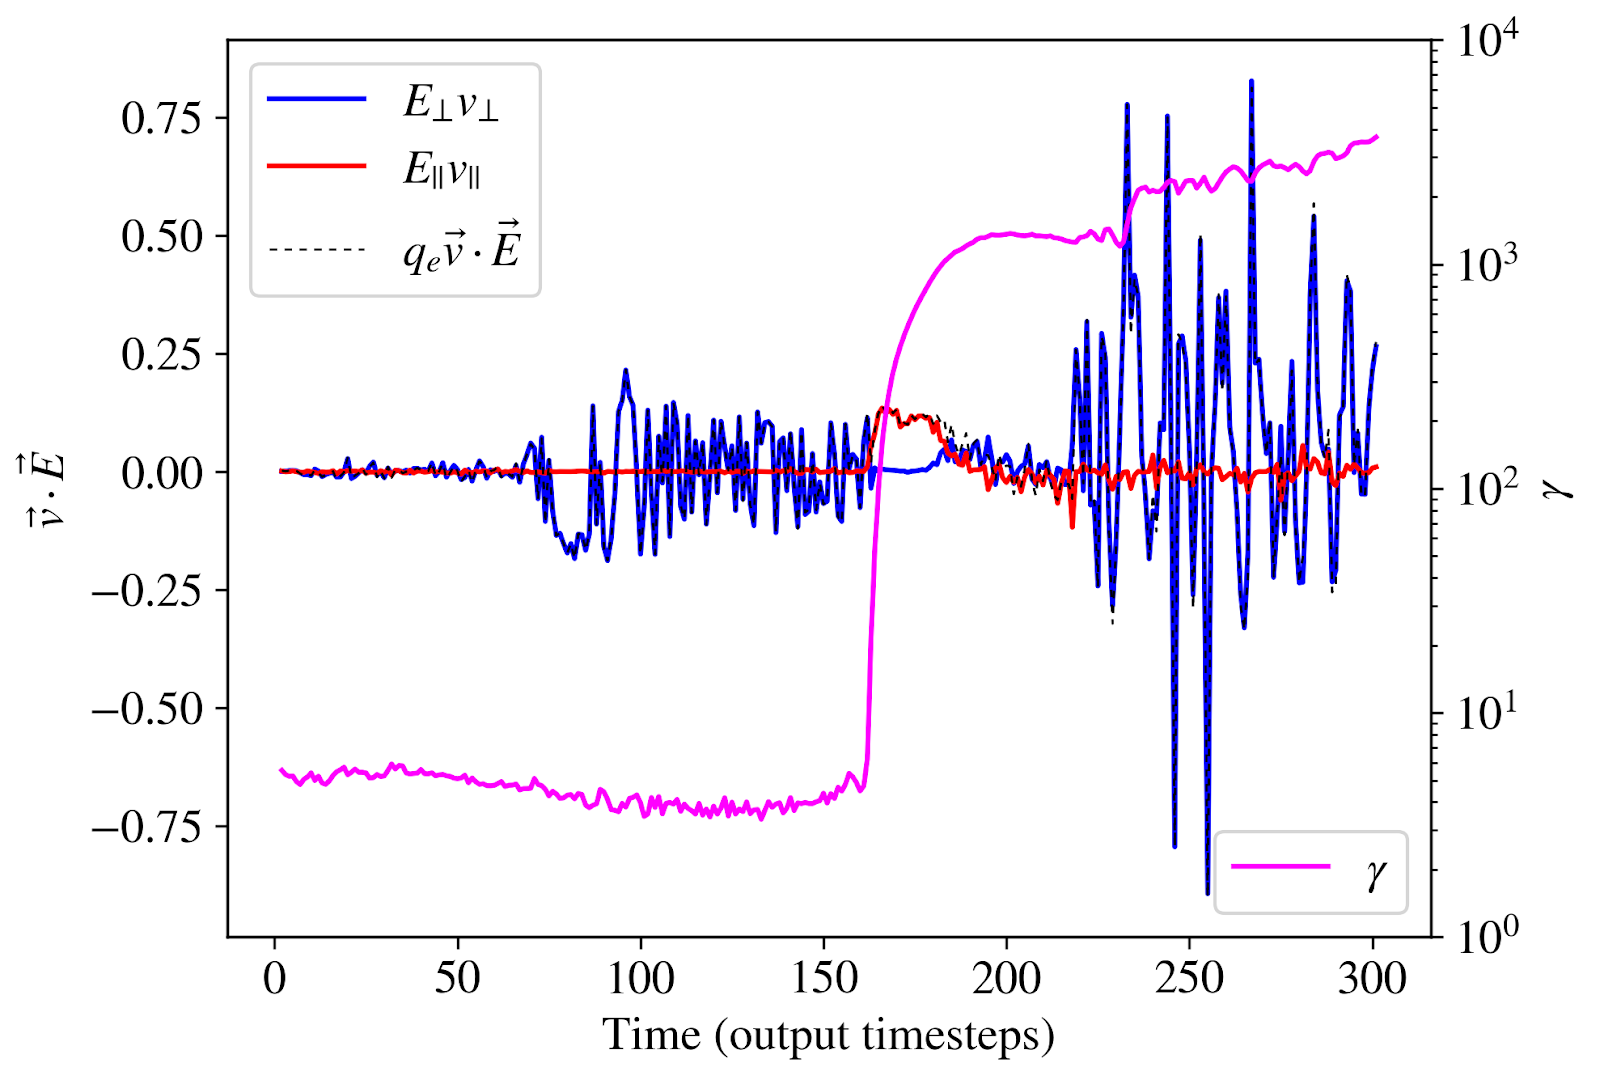
\includegraphics[width=\linewidth]{EdotV.png}
 	%\caption{Evolution of a high-energy particle from the triggered simulation with a guide field.  The particle's Lorentz factor is shown in magenta and corresponds to the right vertical axis.  The instantaneous contributions from the parallel and perpendicular electric fields are shown with red and blue, respectively.  We show the sum of perpendicular and parallel components of work with a dashed black line.}
 	%\label{EdotV}
 %\end{figure}
 
 %In order to statistically examine the role of x-point acceleration, we track the detailed trajectories of a large sample of representative particles.  For each particle, we use the time they are first accelerated beyond $\sigma_{e}/2$, $t_{cs}$, to identify a narrow interval in time around the particle's first acceleration episode $t_{cs} - 300 \omega_{p}^{-1}<t<t_{cs} + 300 \omega_{p}^{-1}$.  Over this time interval, we calculate $W_{||}$.  In this way, we are able to explore whether acceleration at an x-point by a parallel electric field is indeed necessary for a particle to reach highly relativistic energies.  We show in Figure \ref{wpar_hist} a 2d histogram of $W_{||}/W$ during the particles' first acceleration episode vs. particle final energy.  We see that almost all of the particles at the highest energies ($\gamma > 1000$) have $W_{||}/W > 0.5$.  However a large $W_{||}/W$ does not guarantee that the particle will have a large final energy.  In other words, when a particle interacts with an x-point, it will end up with a Lorentz factor of $100-1000$.  After this initial acceleration, other channels for acceleration associated with $W_{\bot}$ become available to the particle and it has a chance to gain even more energy if it encounters fast-moving overdense structures (e.g., plasmoids, outflows) that it can bounce off of in a Fermi-type process.  In this way, we can understand pre-acceleration at an x-point as a necessary but not sufficient condition for a particle to reach the highest energies we see in the system.
 
 % \begin{figure}[htp]
  	
  %	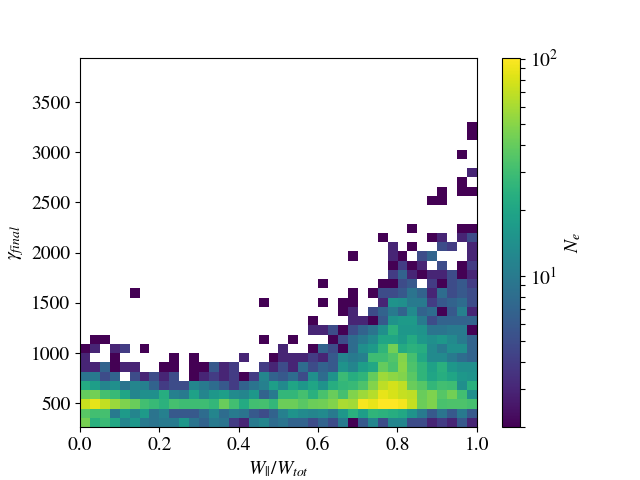
\includegraphics[width=\linewidth]{wpar_untrig.png}
  %	\caption{2d histogram of fractional work done by the parallel electric field during the particle's first acceleration episode vs. particle final energy.  We find that almost all of the highest energy particles ($\gamma > 1000$) are first accelerated by a parallel electric field ($W_{||}/W > 0.5$)}
  %	\label{wpar_hist}
  %\end{figure}


%\section{Implications}
%more x-points / plasmoids lead to harder spectra (Figure \ref{2x2_timespec})
%\begin{figure*}[!h]
%	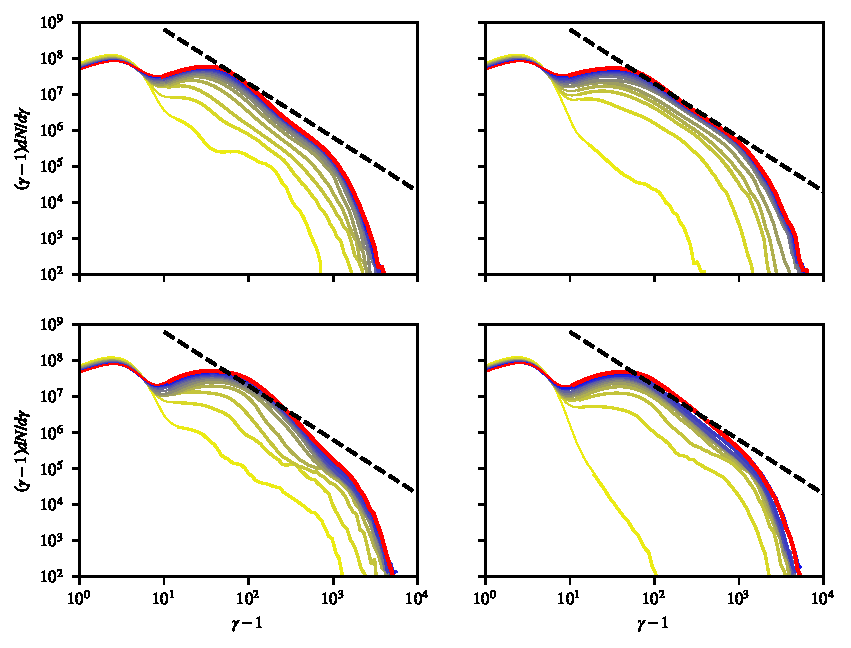
\includegraphics[width=\linewidth]{2x2_timespec.pdf}
%	\caption{Time evolution of electron energy spectra for our four simulations.  Time increases from yellow to blue, and the final snapshot is depicted with a red line.
%	}
%	\label{2x2_timespec}
%\end{figure*}



%an undisturbed current sheet that can fracture over its entire length will produce harder spectra (untriggered) due to the increased number of x-points and plasmoid mergers.  Thinner sheets that fracture more will have harder spectra (or in appendix?)

%anything that suppresses secondary tearing will reduce the amount of particle acceleration (temperature, guide fields).  Suppressing secondary tearing will result in negligible acceleration in the limit of large domains

\section{Test Particles}
In order to more thoroughly test our finding that non-thermal acceleration is largely controlled by x-points, we include in a populations of test particles that only feel certain components of $E_{||}$.  These particles are evolved simultaneously to the normal particles but do not deposit their currents onto the grid.  We use two sets of test particles to explore the energization mechanism of electrons.  One set of test particles does not feel any electric fields parallel to magnetic fields (i.e., $W_{||}=0$), and the other set does not feel any z-component (out-of-plane) of $E_{||}$ field.  We make this distinction for the following reason: when the guide field is high and suppresses the secondary tearing mode, the edges of the outflow show a significant and structured $\vec{E}\cdot\hat{b}$ that is dominantly in the $\pm \hat{x}$ direction (along the outflow) .  Particles that interact with the outflow are energized by this parallel electric field and accelerate to moderate energies.  In fact, these particles make up most of the particles that end up in the thermal peak of the spectrum.  The behavior of $\vec{E}\cdot\hat{b}$ in the vicinity of the primary x-point, however, is significantly different.  As previously discusses, the electric field here is dominantly in the $\hat{z}$ direction, as is $\hat{b}$, resulting in a strong unidirectional $E_{||}$ in the z-direction.  Because of this, we can effectively use test particles to explore the importance of these parallel electric fields (i.e., in the outflow along $\hat{x}$ or near the x-point along $\hat{z}$) to the spectrum of high-energy particles.

\begin{figure*}[htp] 
	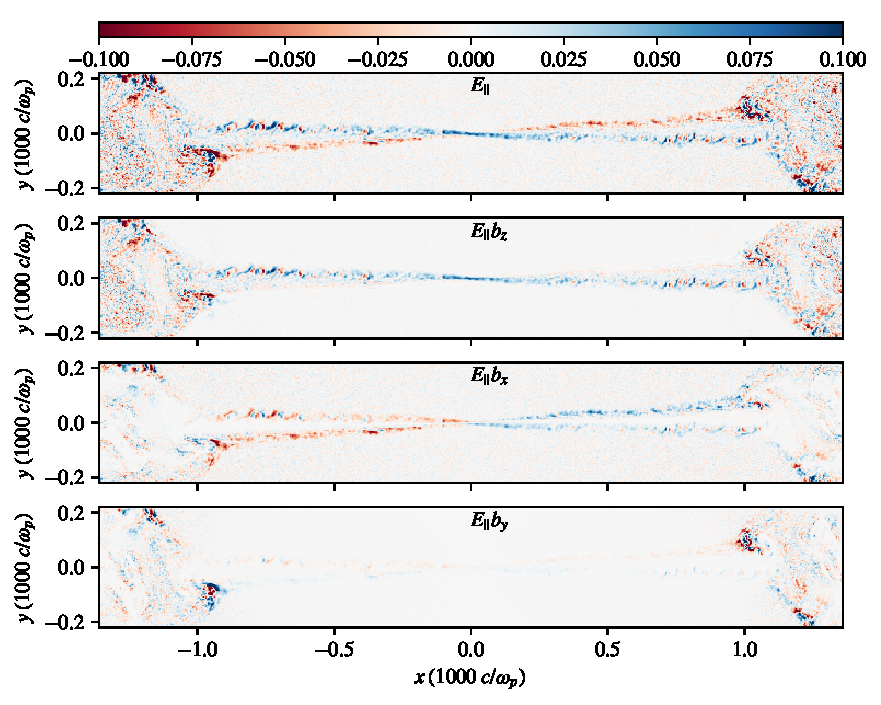
\includegraphics[width=\linewidth]{testing_singleplot_flds.pdf}
	\caption{Profiles of the parallel electric field (top), decomposed into its Cartesian components (bottom three).}
	\label{edotb_comps}
\end{figure*}

\begin{figure}[htp] 
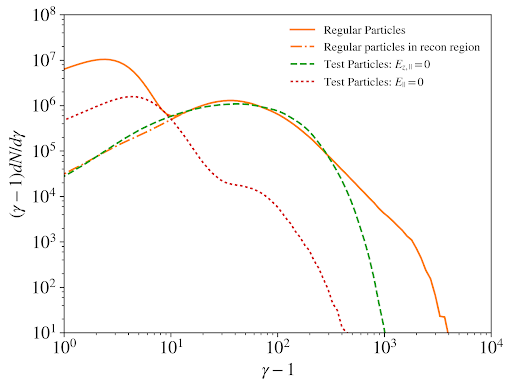
\includegraphics[width=\linewidth]{testspec.png}
\caption{Spectra of different populations of particles.  The regular particle spectrum is shown in orange, the solid line corresponds to the spectrum of particles throughout the entire simulation domain while the dash-dot line shows the spectrum from the reconnection region.  The green dashed line shows the spectrum of test particles that do not experience parallel electric fields in the z-direction and the dotted red line shows the spectrum of particles that do not experience any parallel electric fields.  The spectra for test particles are computed only in the reconnection region.}
\label{testprtl_spec}
\end{figure}




\section{conclusions}
 

\section{Appendix A: Sheet Thickness}\label{thickness_app}
Explore how the current sheet thickness affects the number of x-points per unit length, and hence energy spectra in an untriggered setup (probably in guide field case, probably in no guide field case, secondary plasmoid formation causes fracturing all over anyways and we have a similar number of x-points per unit length)
\section{Appendix B: Box Size}\label{box_size}
Look at case of triggered vs. untriggered as function of boxsize (with guide field), should see a much steeper dependence of triggered case as opposed to untriggered

\FloatBarrier

\bibliography{david_bib}
\bibliographystyle{apj}


\end{document}